% !TeX spellcheck = en_US
% !TeX encoding = UTF-8
\documentclass{beamer}

\mode<presentation> { \usetheme{Madrid} }

\usepackage{graphicx, graphics}
\usepackage[notocbib]{apacite}
\usepackage[style=iso]{datetime2}
\usepackage{enumerate}
\DeclareGraphicsExtensions{.pdf, .png, .jpg, .gif}

\AtBeginSection[]
{
    \begin{frame}
        \vfill
        \centering
        \begin{beamercolorbox}[sep=8pt, center, shadow=true, rounded=true]{title}
            \usebeamerfont{title}
            \insertsectionhead
            \par
        \end{beamercolorbox}
        \vfill
    \end{frame}
}

\title[Periodontitis]{Periodontitis}

\author[Seunghoon Kim \and Jaewoong Lee]
{
    Seunghoon Kim
    \and
    Jaewoong Lee
    \and
    Semin Lee
}

\institute[UNIST]
{
    Ulsan National Institute of Science and Technology
    \medskip
    \newline
    \textit{jwlee230@unist.ac.kr}
}
\date{\today}

\begin{document}
    \begin{frame}
        \titlepage
    \end{frame}

    \begin{frame}
        \frametitle{Overview}
        \tableofcontents
    \end{frame}

    \section{Introduction}
    \begin{frame}
        \frametitle{Microbiome}

        \begin{itemize}
            \item Microbiota: the micro-organisms which live inside \& on humans \cite{microbiome1}
            \item Microbiome: about $10^{13}$ micro-organisms whose which collective genome \cite{microbiome2}
        \end{itemize}

        \begin{figure}
            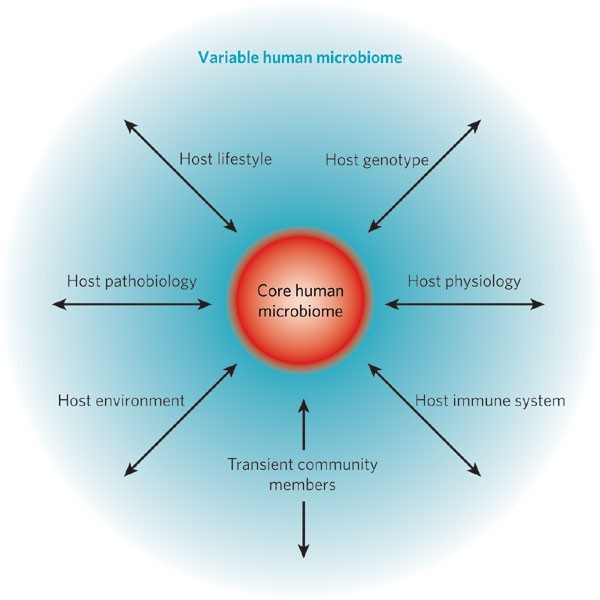
\includegraphics[width=0.3 \linewidth]{figures/microbiome.jpg}
            \caption{Concept of a core human microbiome \protected \cite{microbiome1}}
            \label{fig:microbiome}
        \end{figure}
    \end{frame}

    \begin{frame}
        \frametitle{rRNA}

        \begin{itemize}
            \item Ribosomal RNA
            \item Well-known as a key to phylogeny \cite{rRNA1}
        \end{itemize}
    \end{frame}

    \begin{frame}
        \frametitle{Periodontitis (Periodontal disease)}

        \begin{itemize}
            \item CAL (Clinical Attachment Loss) \& BL (Bone Loss) \cite{periodontitis1}
            \item Risk Factors \cite{periodontitis2}
            \begin{enumerate}
                \item Smoking
                \item Diabetes
                \item Genetic factor
                \item Host response
            \end{enumerate}
        \end{itemize}
    \end{frame}

    \section{Materials}
    \begin{frame}
        \frametitle{16S rRNA Sequencing}

        \begin{itemize}
            \item 100 Healthy people
            \item 50 Chronic periodontitis -- Early
            \item 50 Chronic periodontitis -- Moderate
            \item 50 Chronic periodontitis -- Severe
        \end{itemize}
    \end{frame}

    \section{Methods}
    \begin{frame}
        \frametitle{QIIME2 Workflow}

        \begin{figure}
            \centering
            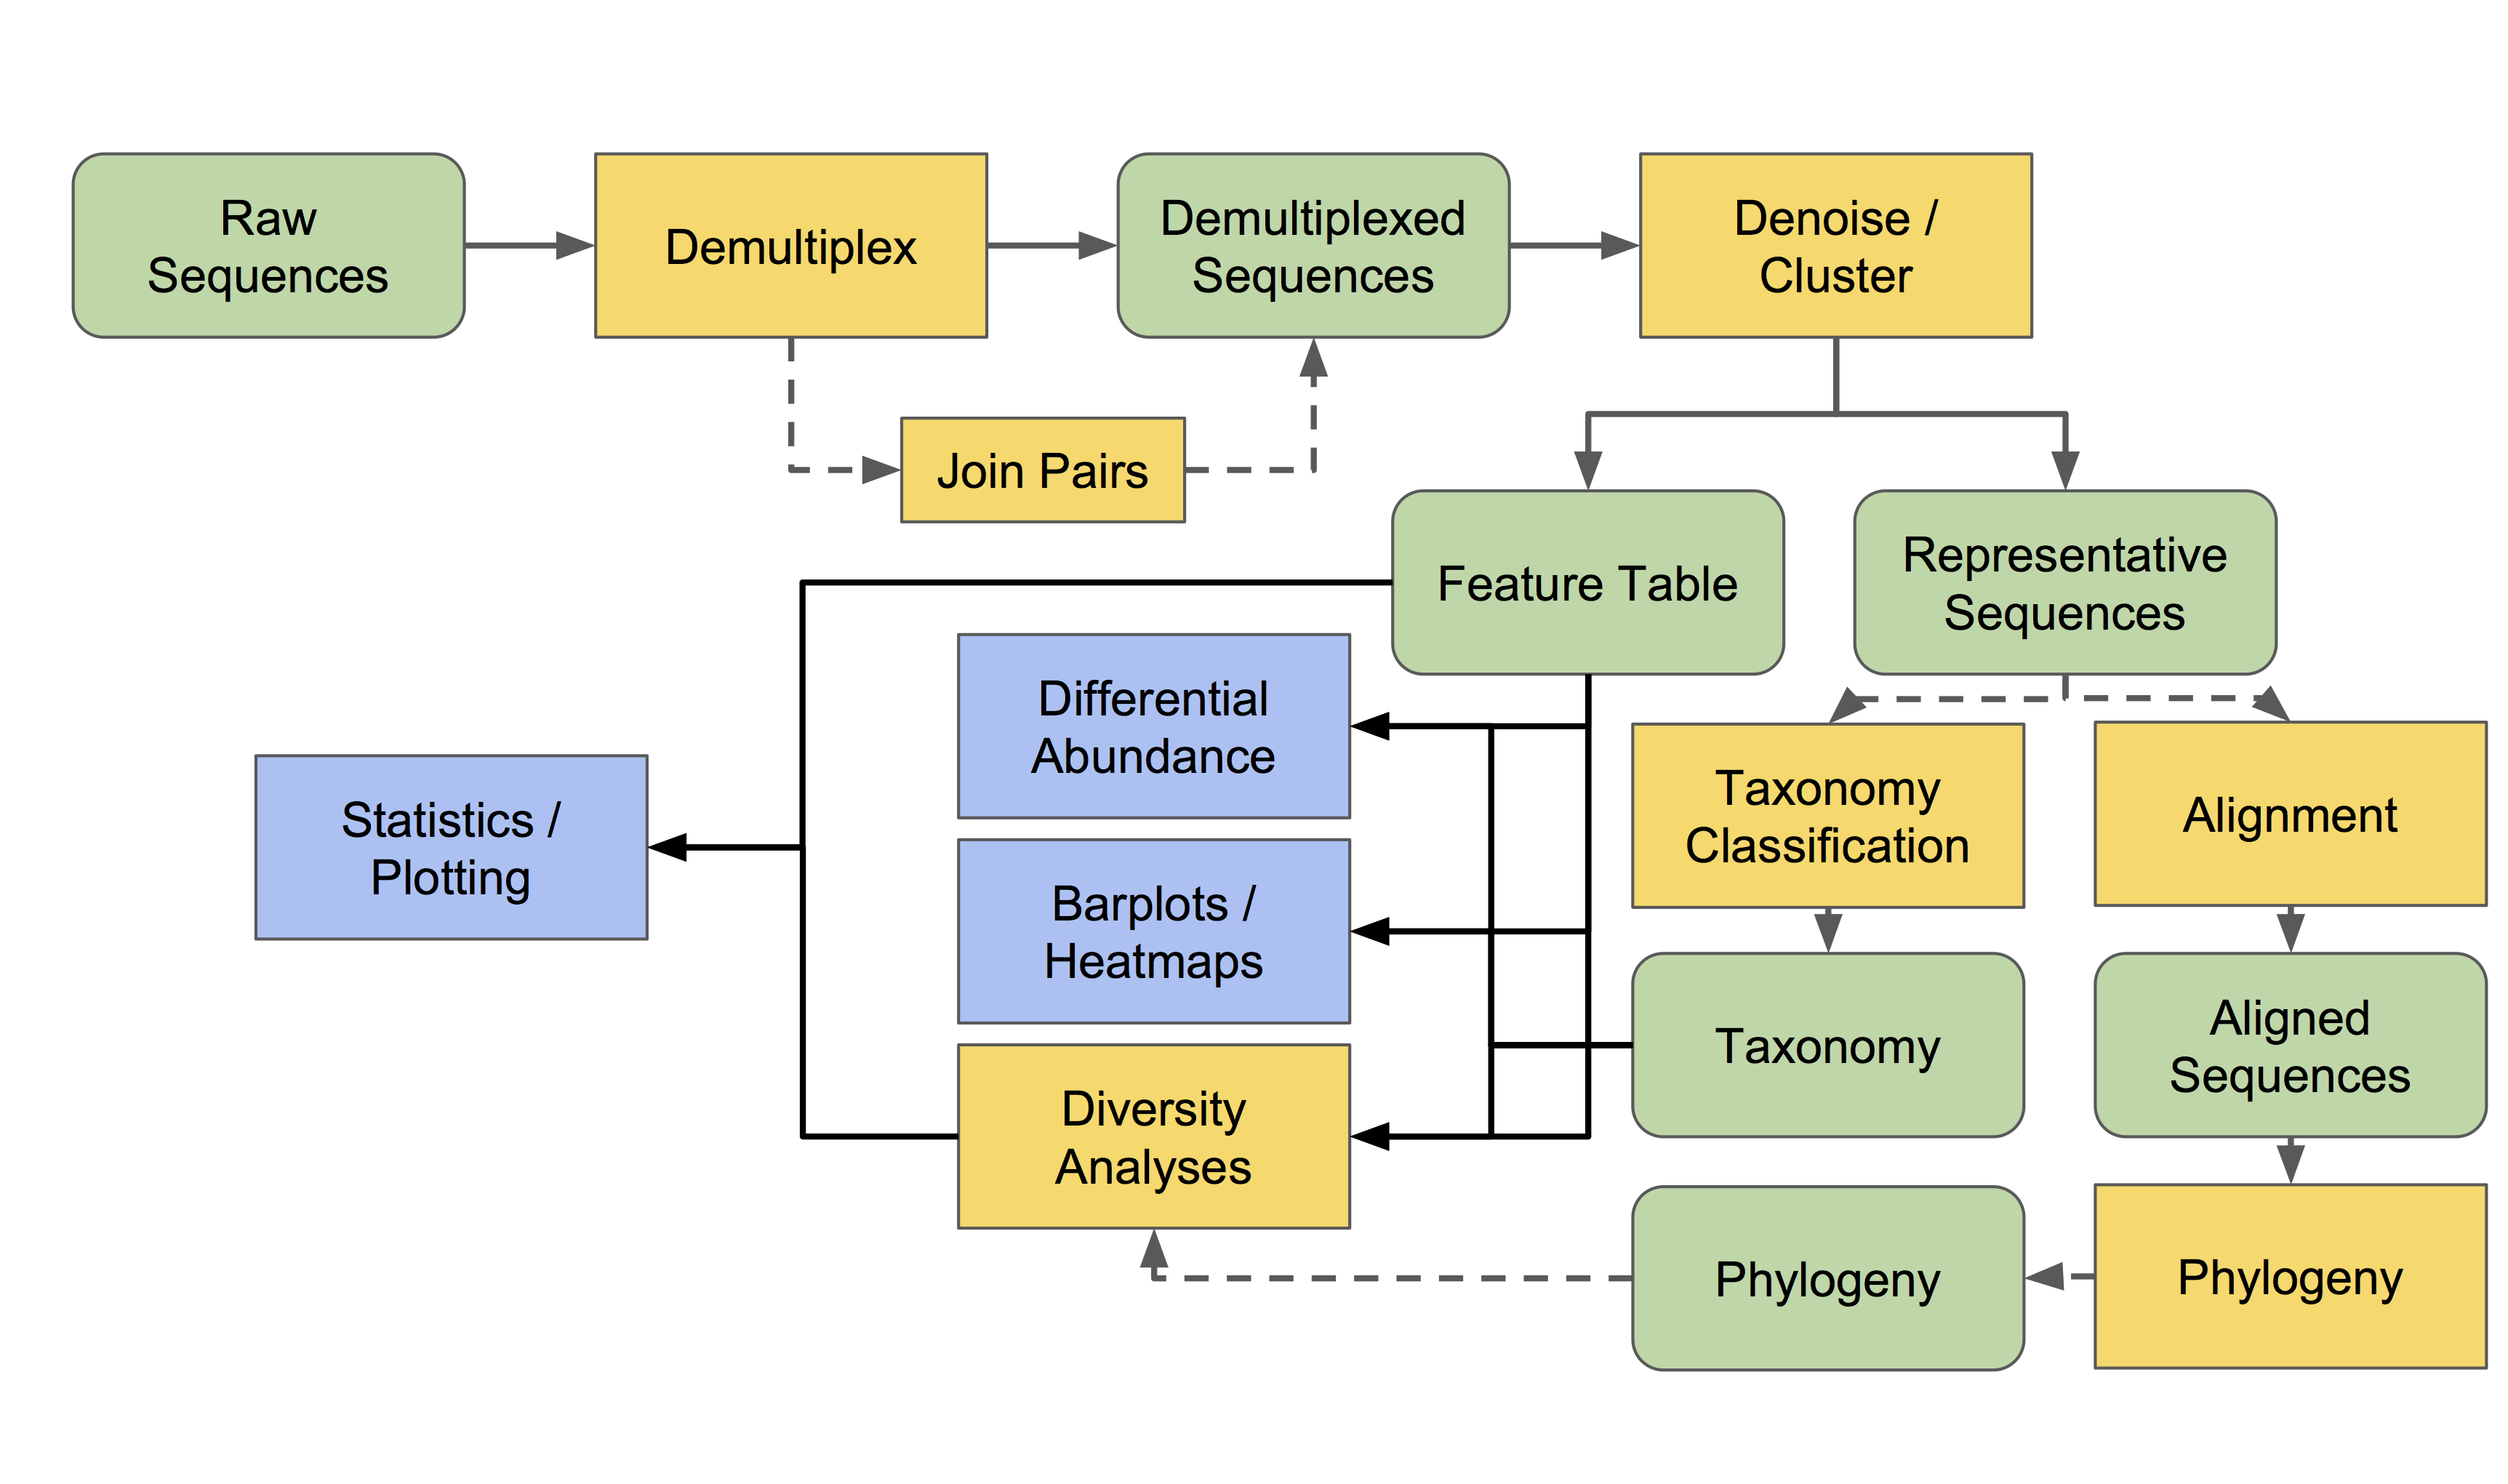
\includegraphics[width=0.7 \linewidth]{figures/qiime.png}
            \caption{QIIME2 Workflow \protect\cite{qiime1, qiime2}}
            \label{fig:qiime}
        \end{figure}
    \end{frame}

    \begin{frame}
        \frametitle{Denoising techniques}

        \begin{itemize}
            \item DADA2: Amplicon Sequence Variants (ASVs) \cite{DADA1}
            \item Deblur: Operational Taxonomic Units (OTUs) \cite{deblur1}
        \end{itemize}

        \begin{figure}
            \centering
            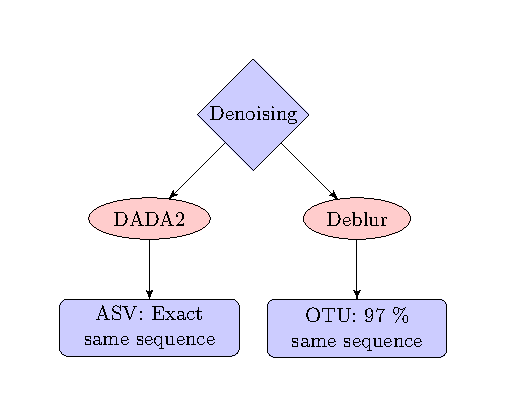
\includegraphics[width=0.4 \linewidth]{figures/denoising/denoising.pdf}
            \caption{Denoising Techniques}
            \label{fig:denoising}
        \end{figure}
    \end{frame}

    \begin{frame}
        \frametitle{Taxonomy Classification}

        \begin{itemize}
            \item Greengenes (GG) \cite{greengenes1}
            \item SILVA \cite{silva1}
        \end{itemize}

        \begin{figure}
            \centering
            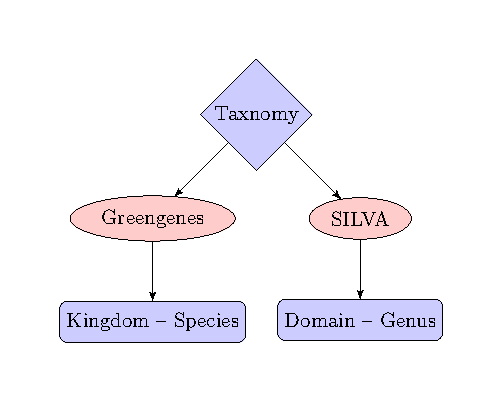
\includegraphics[width=0.4 \linewidth]{figures/taxonomy/taxonomy.pdf}
            \caption{Taxonomy Classification}
            \label{fig:taxonomy}
        \end{figure}

        “A \textbf{higher} performance at taxonomic levels above \textit{genus} level; but performance appears to drop at \textit{species} level” \cite{performance1}
    \end{frame}

    \begin{frame}
        \frametitle{Merging Denosing and Taxonomy Classification}

        Merging multiple IDs (ASVs and OTUs) into one, which have:
        \begin{itemize}
            \item Different IDs.
            \item Identified as same taxonomy.
        \end{itemize}

        \begin{figure}
            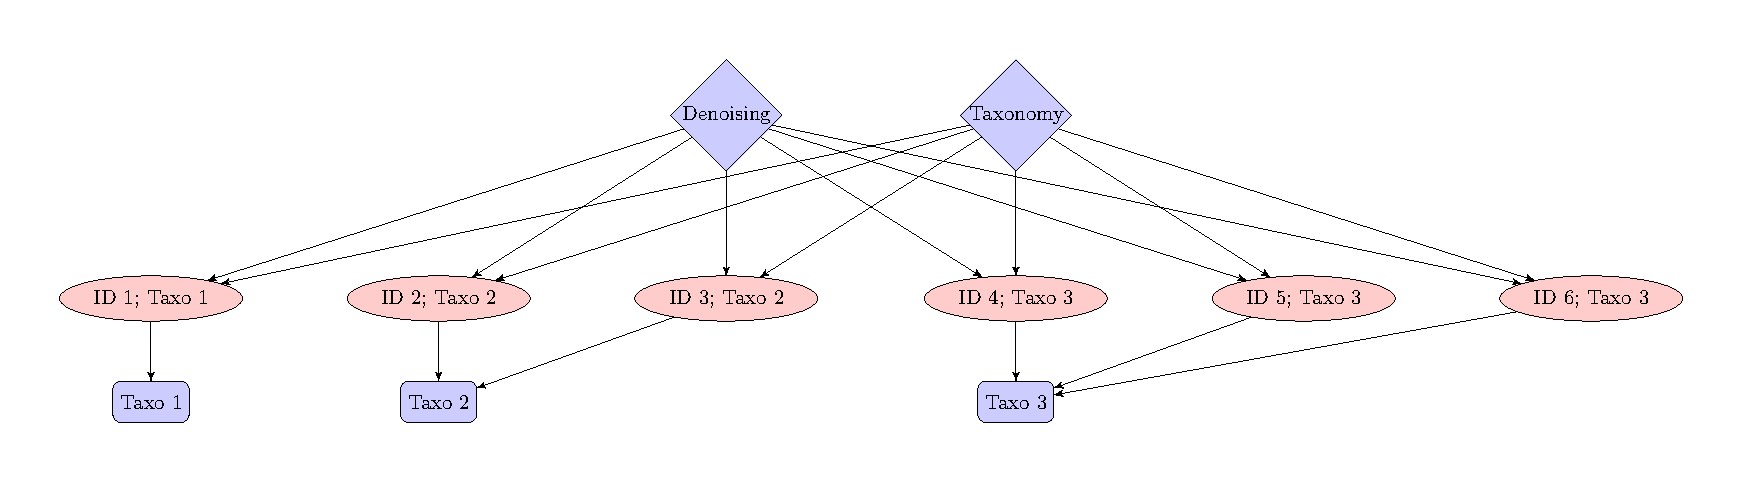
\includegraphics[width=0.6 \linewidth]{figures/Merging/merging.pdf}
            \caption{Example Diagram for Merging Denosing and Taxonomy Classification}
        \end{figure}
    \end{frame}

    \begin{frame}
        \frametitle{Rarefaction}

        \begin{itemize}
            \item a statistical method of estimating the number of species expected in a random sample which taken from a collection \cite{rarefaction1}
            \item allows comparisons of the species richness among communities
            \item a good choice for normalization \cite{rarefaction2}
        \end{itemize}
    \end{frame}

    \begin{frame}
        \frametitle{Alpha- \& Beta-diversity}

        \begin{itemize}
            \item alpha-diversity: the richness of taxa at a single community
            \item beta-diversity: the taxonomic differentiation between communities
        \end{itemize}
    \end{frame}

    \begin{frame}
        \frametitle{Alpha-diversity}

        \begin{itemize}
            \item Shannon's diversity index: a quantitative measure of community richness
            \item Observed Features: a qualitative measure of community richness
            \item Faith's Phylogenetic Diversity: a qualitative measure of community richness which incorporates phylogenetic relationship between the features
            \item Evenness: a measure of community evenness
        \end{itemize}
        \cite{qiime1, qiime2}
    \end{frame}

    \begin{frame}
        \frametitle{Beta-diversity}

        \begin{itemize}
            \item Bray-Curtis distance: a quantitative measure of community dissimilarity
            \item Jaccard distance: a qualitative measure of community dissimilarity
            \item Unweighted UniFrac distance: a qualitative measure of community dissimilarity which incorporates phylogenetic relationships between the features
            \item Weighted UniFrac distance: a quantitative measure of community dissimilarity which incorporates phylogenetic relationship between the features
        \end{itemize}
        \cite{qiime1, qiime2}
    \end{frame}

    \begin{frame}
        \frametitle{ANCOM}

        \begin{itemize}
            \item Analysis of composition of microbiomes
            \item ANCOM can be used for analyzing the composition of microbiomes in multiple populations \cite{ANCOM1}
            \item Differential abundance testing
        \end{itemize}

        \begin{figure}
            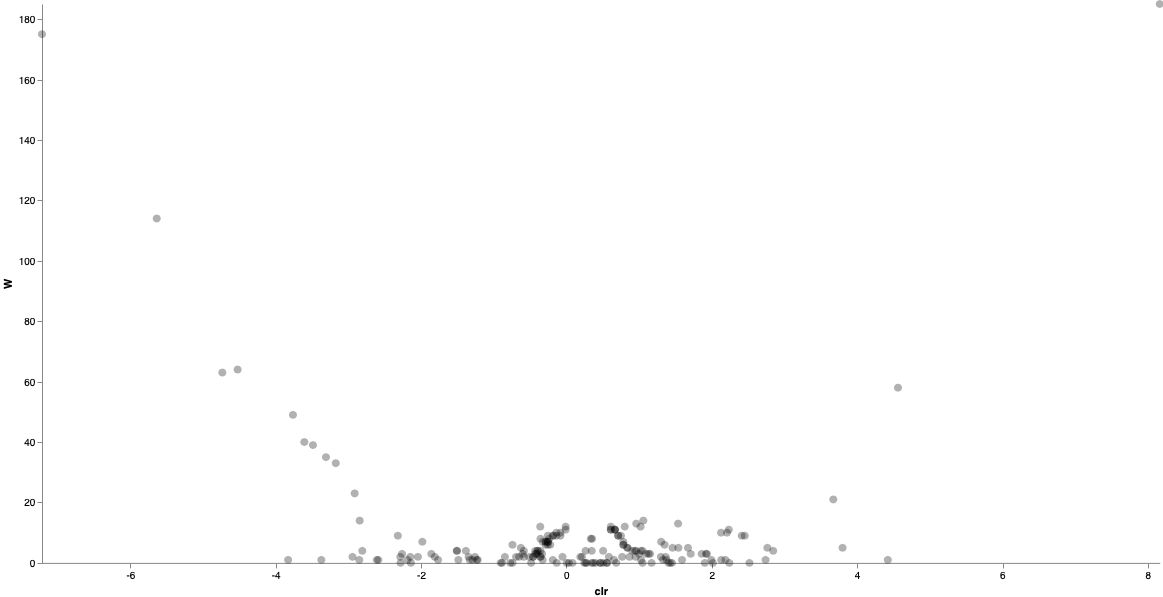
\includegraphics[width=0.3 \linewidth]{figures/ANCOM/example.png}
            \caption{Example ANCOM Volcano Plot \protect\cite{qiime1, qiime2}}
        \end{figure}

        \begin{itemize}
            \item clr: Centered log Ratio
            \item W: a count of the number of sub-hypothesis which have passed for given species
        \end{itemize}
    \end{frame}

    \begin{frame}
        \frametitle{Python Packages}

        \begin{itemize}
            \item Pandas \cite{pandas1}
            \item Scikit-learn \cite{sklearn1}
            \item Matplotlib \cite{matplotlib1, matplotlib2}
            \item Seaborn \cite{seaborn1}
        \end{itemize}
    \end{frame}

    \begin{frame}
        \frametitle{t-SNE}

        \begin{itemize}
            \item t-distributed stochastic neighbor embedding
            \item reveals high-dimensional data a location in two-dimensional map \cite{tSNE1}
        \end{itemize}

        \begin{figure}
            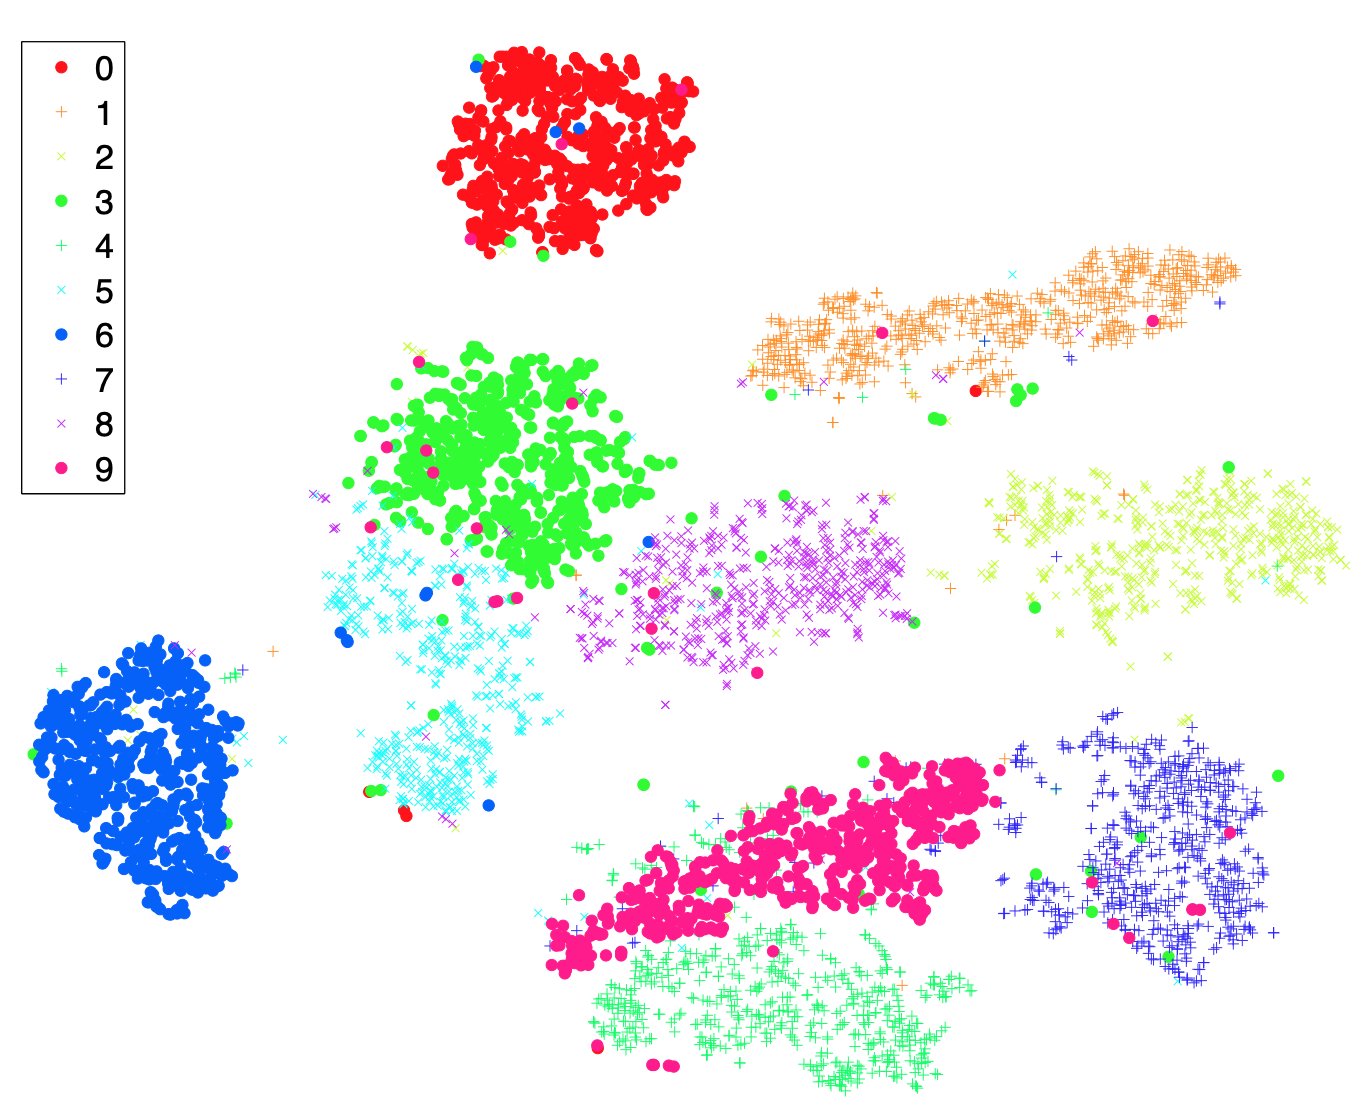
\includegraphics[width=0.4 \linewidth]{figures/tSNE.png}
            \caption{Visualization by t-SNE \protect\cite{tSNE1}}
        \end{figure}
    \end{frame}

    \begin{frame}[allowframebreaks]
        \frametitle{Classification}

        \begin{figure}
            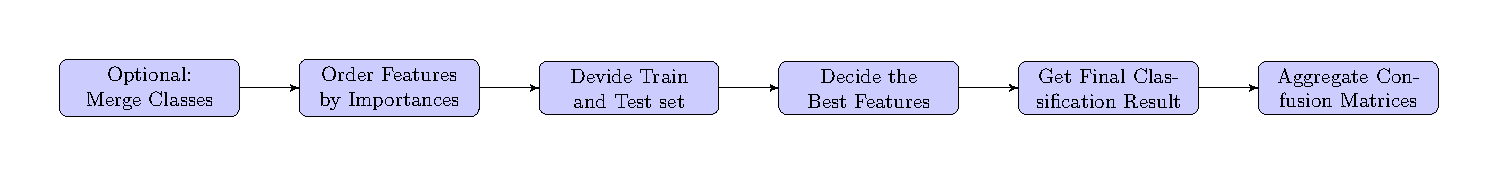
\includegraphics[width=0.8 \linewidth]{figures/Classifier/classifier.pdf}
            \caption{Workflow of Classification}
        \end{figure}

        Classification Metrics:
        \begin{itemize}
            \item Accuracy
            \item Balanced Accuracy
            \item Sensitivity
            \item Specificity
            \item Precision
        \end{itemize}

        \begin{figure}
            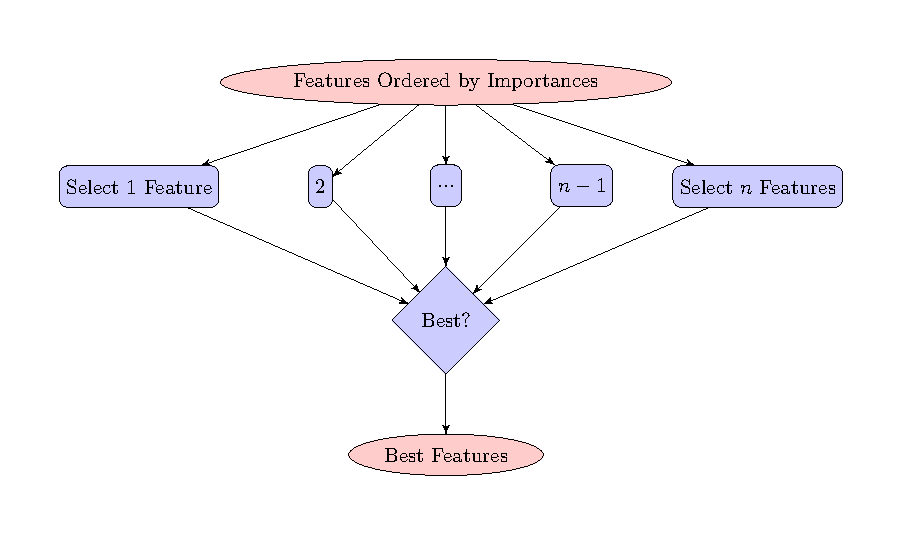
\includegraphics[width=0.8 \linewidth]{figures/Classifier/best.pdf}
            \caption{Deciding the Best Features}
        \end{figure}
    \end{frame}

    \section{Results}
    \begin{frame}
        \frametitle{Quality Filter}

        \begin{figure}
            $\begin{array}{cc}
                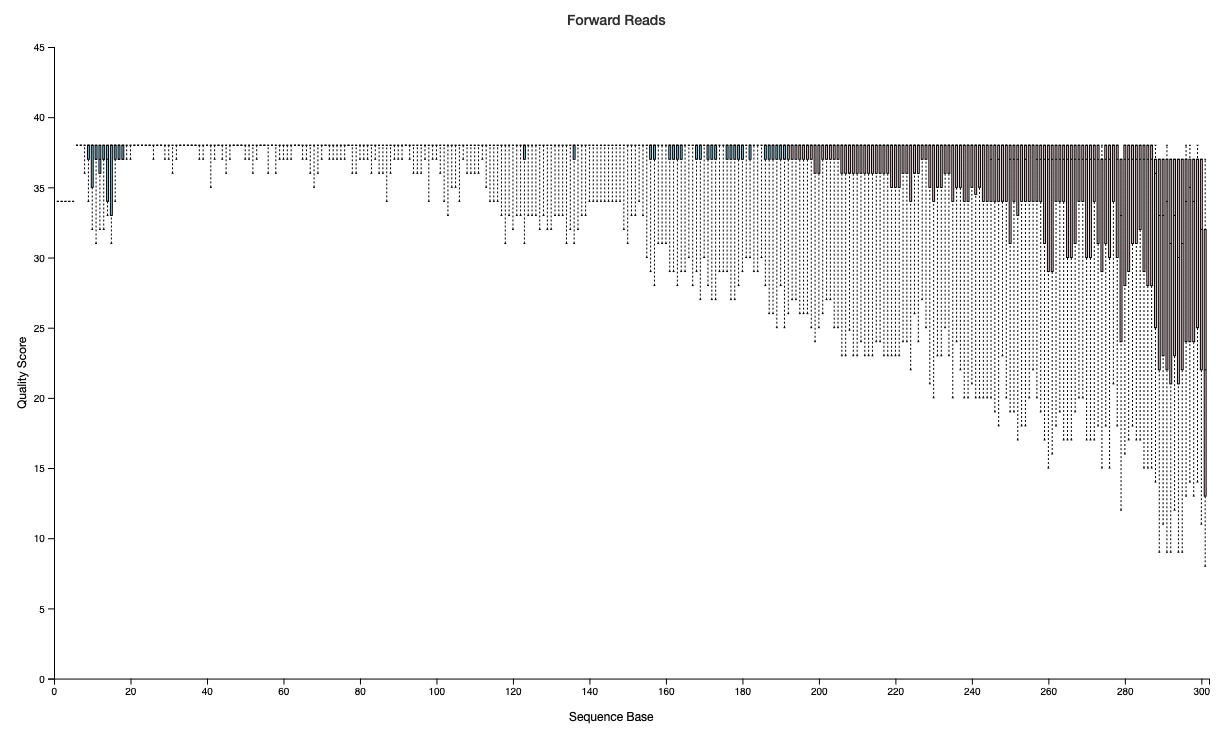
\includegraphics[width=0.4 \linewidth]{figures/QualityFilter/Forward.png}
                &
                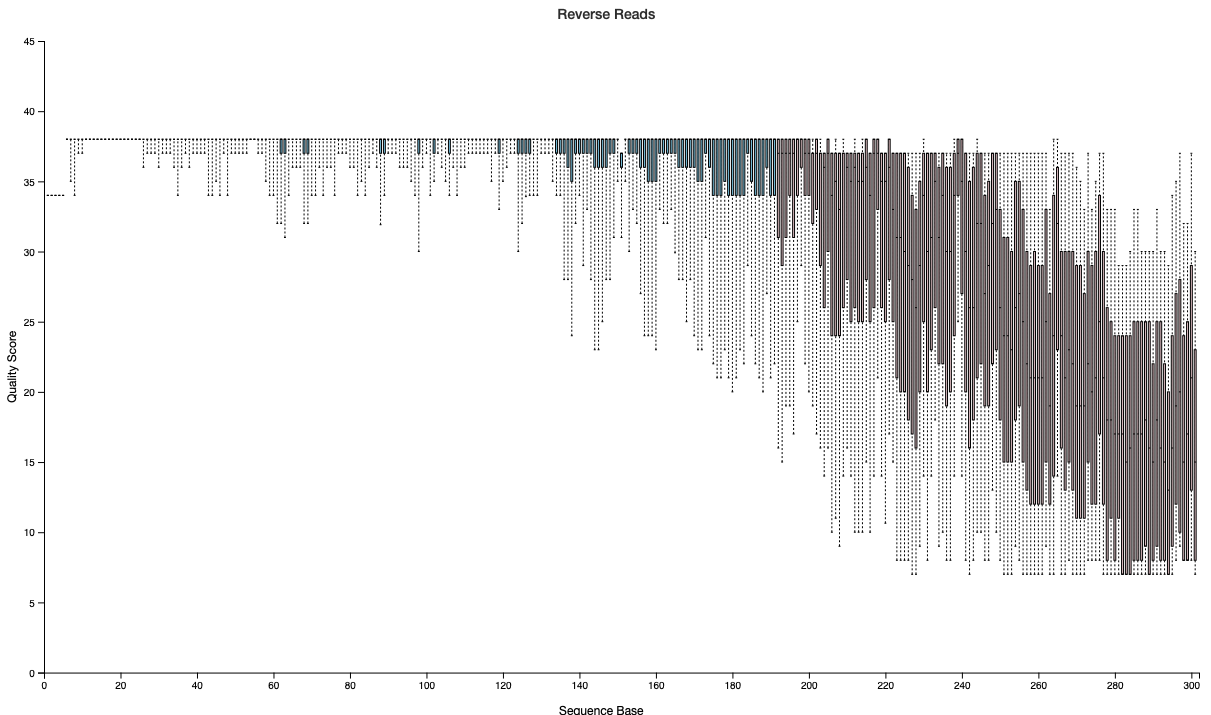
\includegraphics[width=0.4 \linewidth]{figures/QualityFilter/Reverse.png}
                \\
                \mbox{(a) Forward Reads} & \mbox{(b) Reverse Reads}
            \end{array}$
            \caption{Sequence Quality Plot}
        \end{figure}

        $\therefore$ Maximum Sequence Length $n_{forword}$ = 300, $n_{reverse}$ = 265 \\
        $\because$ The longest length which has sequence quality $\ge 30$ at middle.
    \end{frame}

    \begin{frame}
        \frametitle{Rarefaction}

        \begin{figure}
            $\begin{array}{cc}
                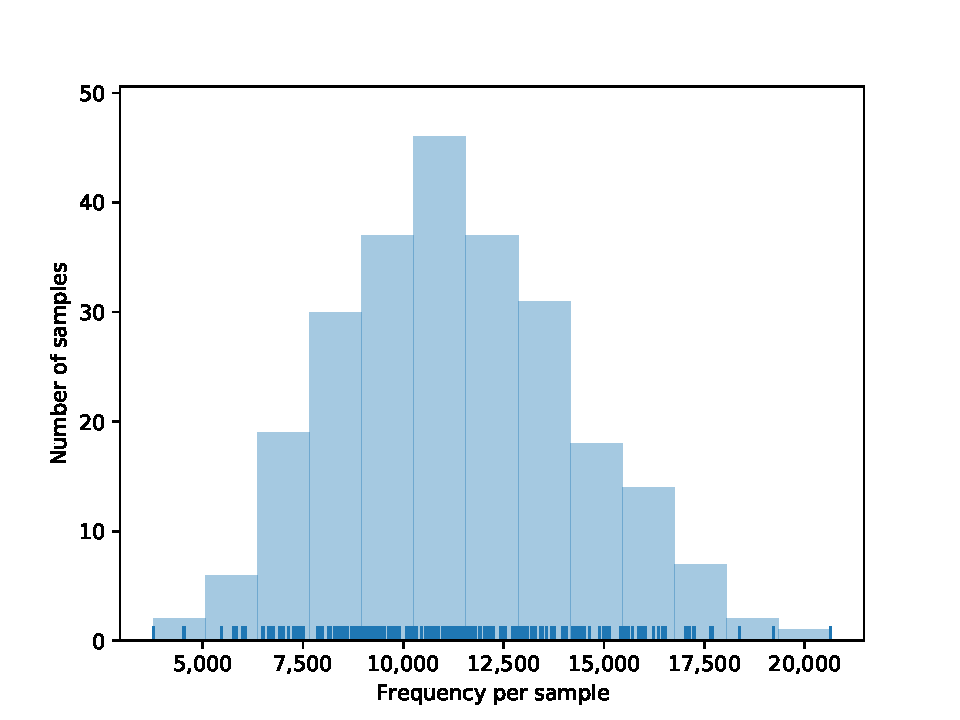
\includegraphics[width=0.4 \linewidth]{figures/Rarefaction/DADA.pdf}
                &
                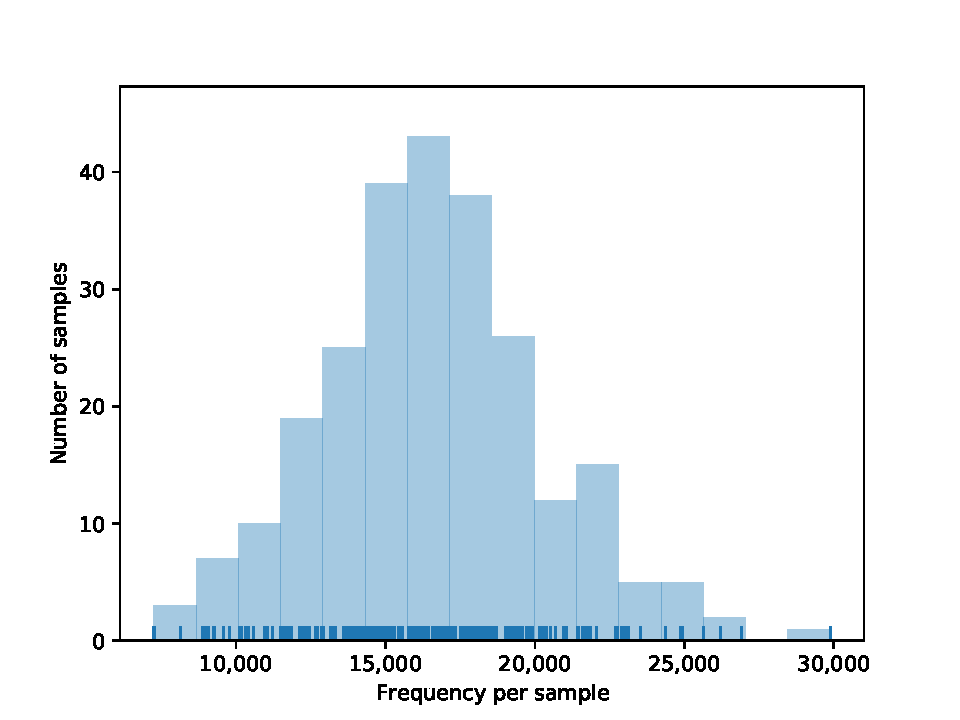
\includegraphics[width=0.4 \linewidth]{figures/Rarefaction/Deblur.pdf}
                \\
                \mbox{(a) DADA2} & \mbox{(b) Deblur} \\
            \end{array}$
            \caption{Frequency per sample}
        \end{figure}

        $\therefore$ p-sampling-depth $n_{DADA2} = 3786$ and $n_{Deblur} = 7253$\\
    \end{frame}

    \begin{frame}[allowframebreaks]
        \frametitle{Alpha-diversity}

        \begin{figure}
            $\begin{array}{cc}
                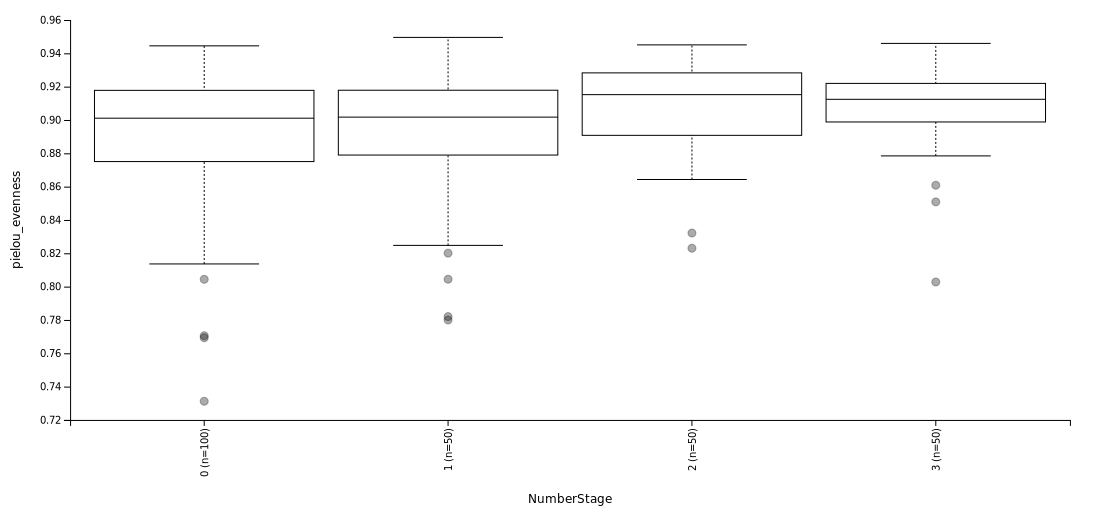
\includegraphics[width=0.4 \linewidth]{figures/AlphaDiversity/DADA2/evenness.png}
                &
                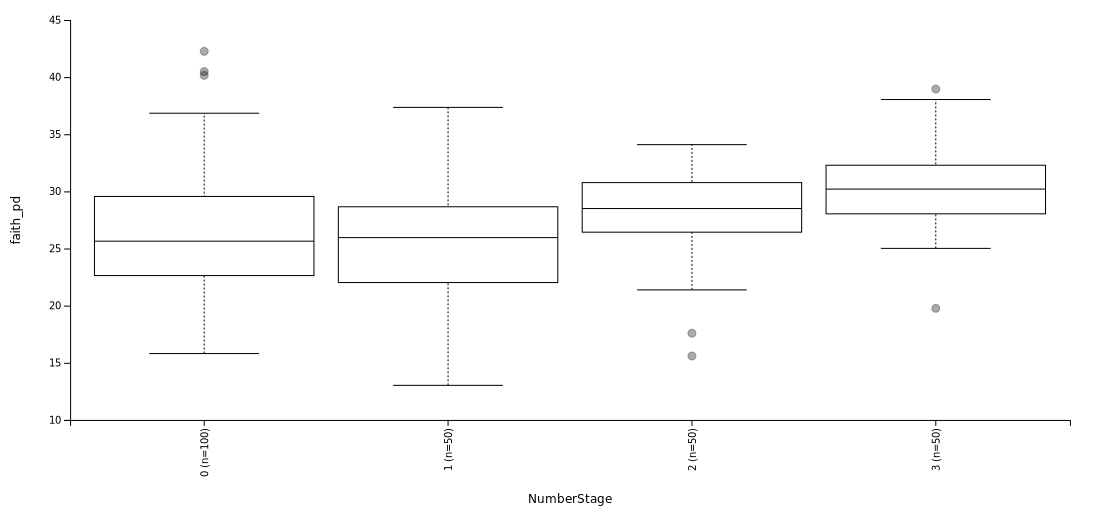
\includegraphics[width=0.4 \linewidth]{figures/AlphaDiversity/DADA2/faith.png}
                \\
                \mbox{(a) Evenness ($p < 0.01$)} & \mbox{(b) Faith PD ($p < 10^{-6}$)} \\

                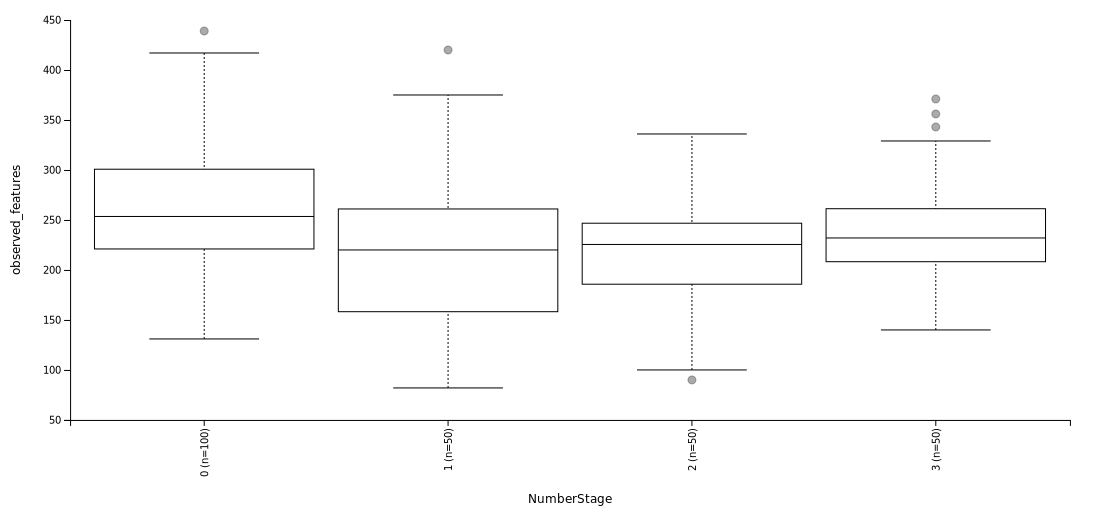
\includegraphics[width=0.4 \linewidth]{figures/AlphaDiversity/DADA2/observed.png}
                &
                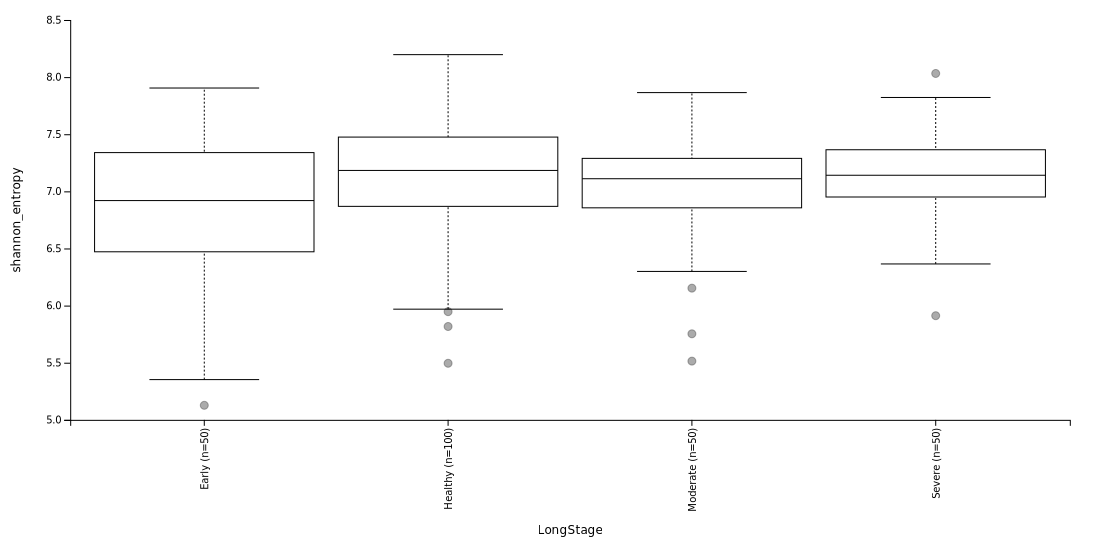
\includegraphics[width=0.4 \linewidth]{figures/AlphaDiversity/DADA2/shannon.png}
                \\
                \mbox{(c) Observed features ($p < 10^{-3}$)} & \mbox{(d) Shannon's diversity ($p > 0.05$)}
            \end{array}$
            \caption{Alpha Diversity from DADA2 with Kruskal-Wallis among All Groups}
        \end{figure}

        \begin{figure}
            $\begin{array}{cc}
                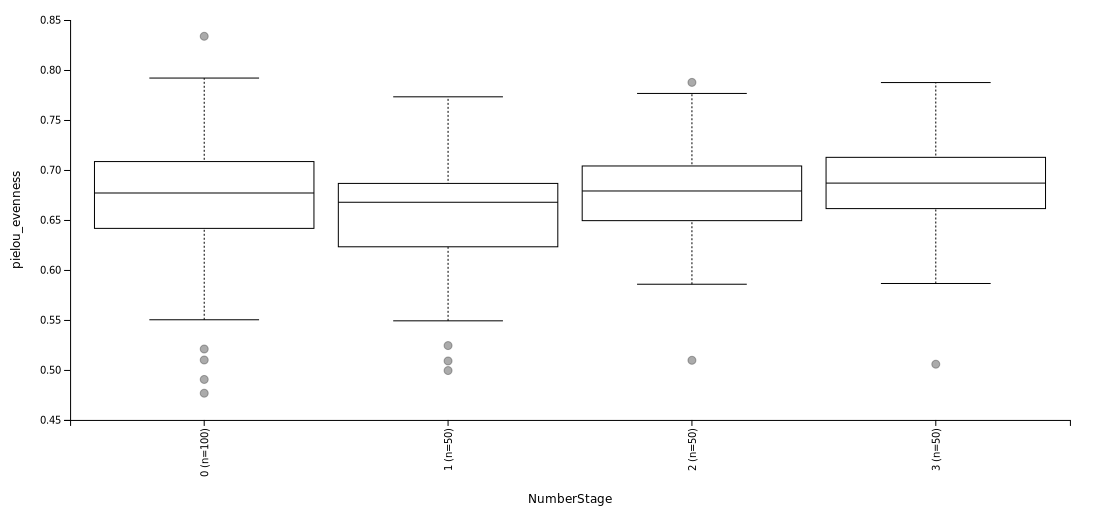
\includegraphics[width=0.4 \linewidth]{figures/AlphaDiversity/Deblur/evenness.png}
                &
                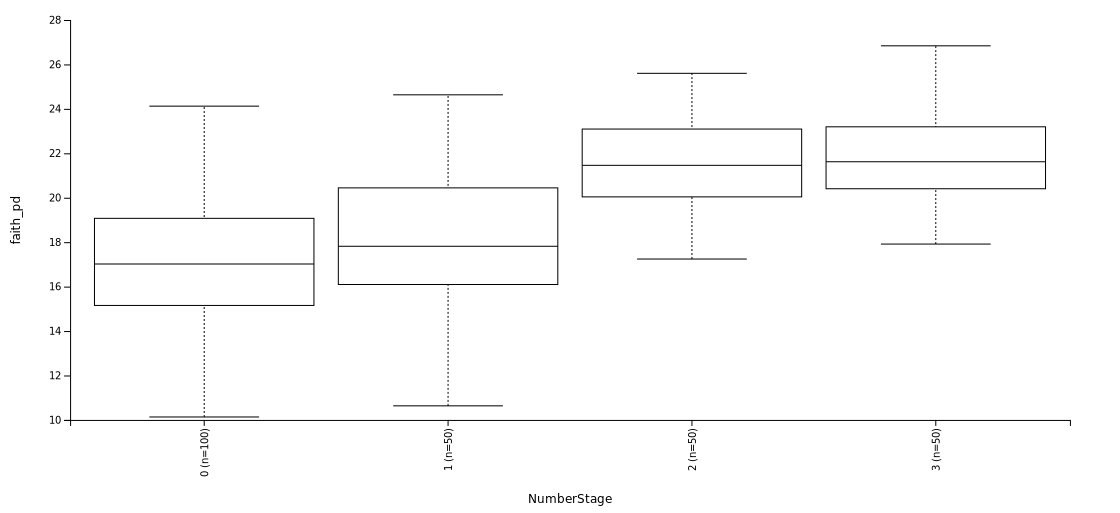
\includegraphics[width=0.4 \linewidth]{figures/AlphaDiversity/Deblur/faith.png}
                \\
                \mbox{(a) Evenness ($p < 0.05$)} & \mbox{(b) Faith PD ($p < 10^{-18}$)} \\

                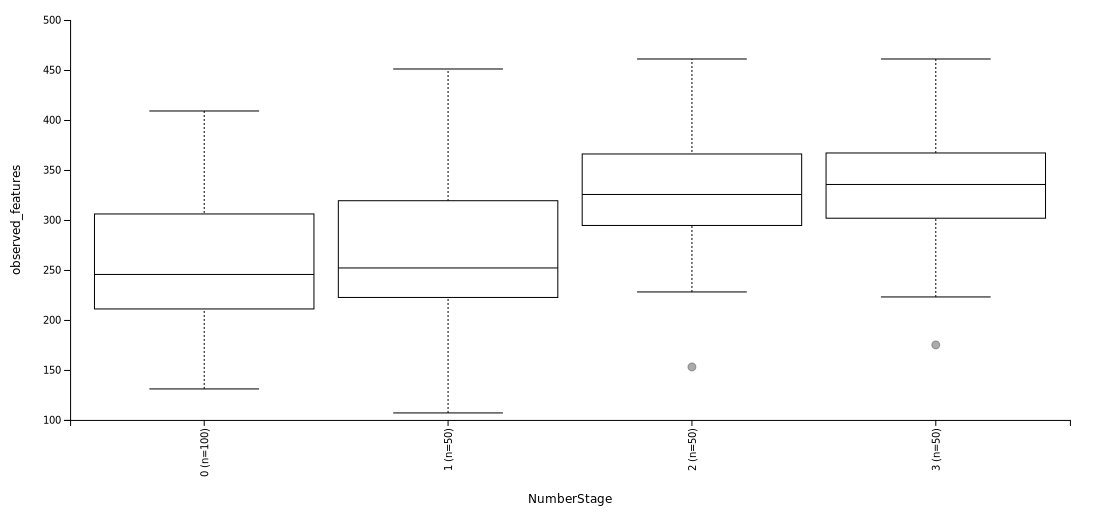
\includegraphics[width=0.4 \linewidth]{figures/AlphaDiversity/Deblur/observed.png}
                &
                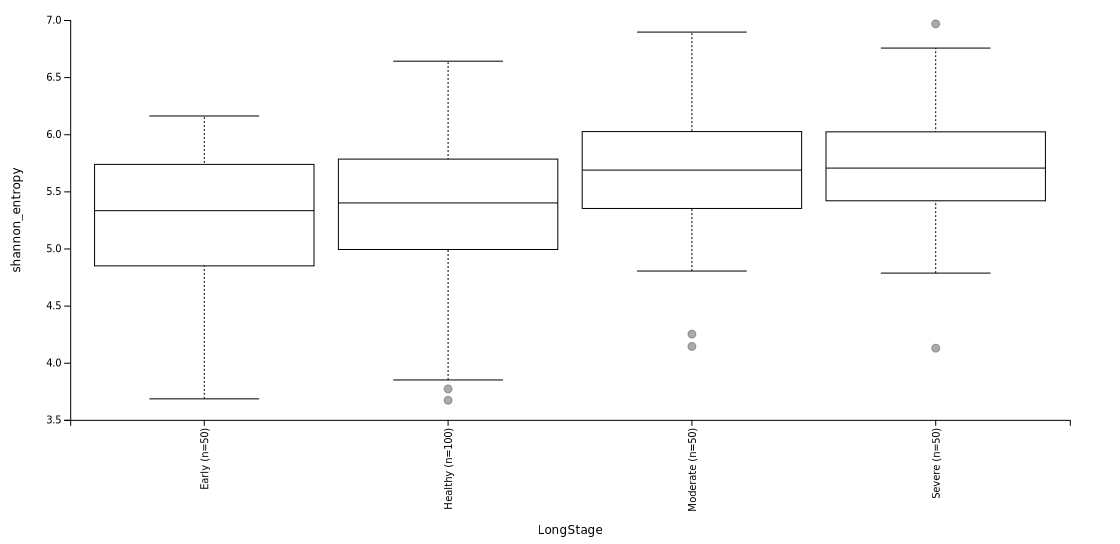
\includegraphics[width=0.4 \linewidth]{figures/AlphaDiversity/Deblur/shannon.png}
                \\
                \mbox{(c) Observed features ($p < 10^{-12}$)} & \mbox{(d) Shannon's diversity ($p < 10^{-4}$)}
            \end{array}$
            \caption{Alpha Diversity from Deblur with Kruskal-Wallis among All Groups}
        \end{figure}
    \end{frame}

    \begin{frame}[allowframebreaks]
        \frametitle{Beta-diversity}

        \begin{figure}
            $\begin{array}{cc}
                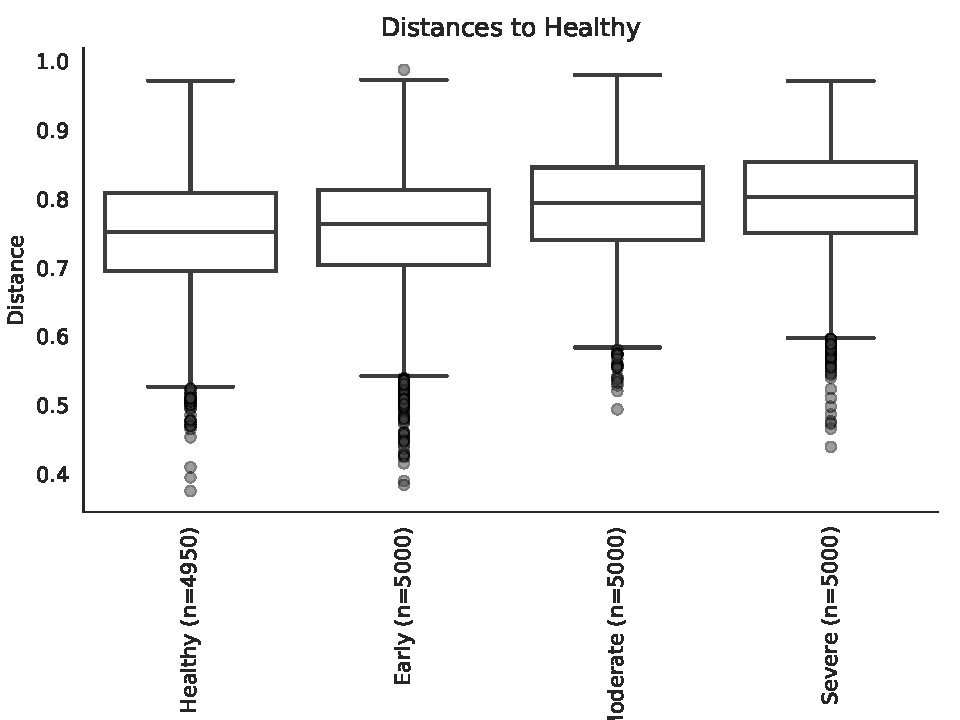
\includegraphics[width=0.25 \linewidth]{figures/BetaDiversity/DADA2/Bray/Healthy.pdf}
                &
                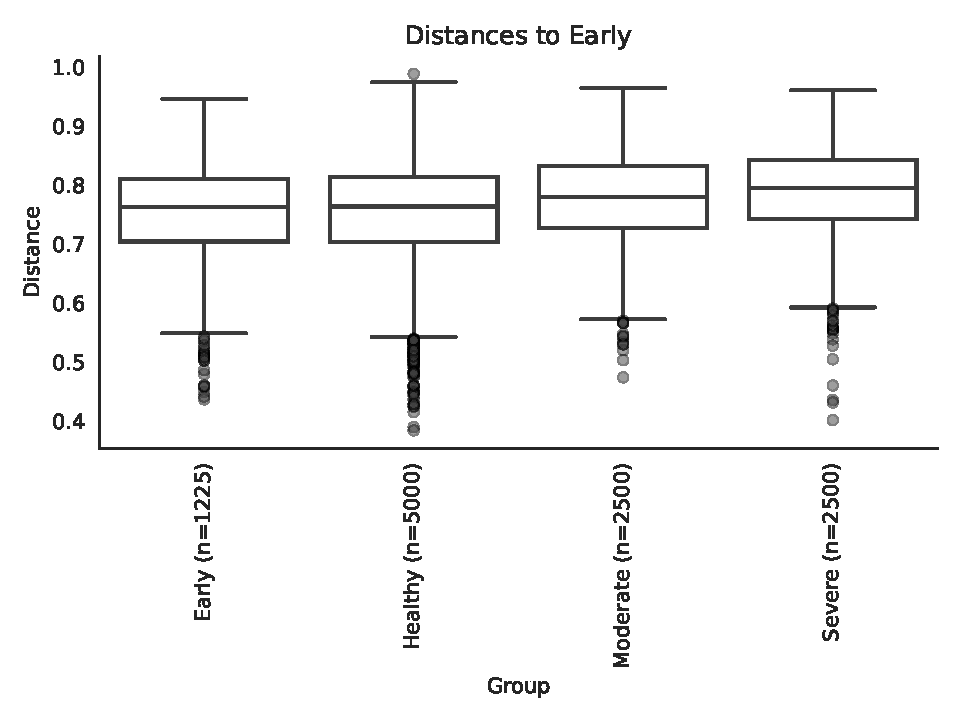
\includegraphics[width=0.25 \linewidth]{figures/BetaDiversity/DADA2/Bray/Early.pdf}
                \\
                \mbox{(a) Healthy} & \mbox{(b) Early} \\

                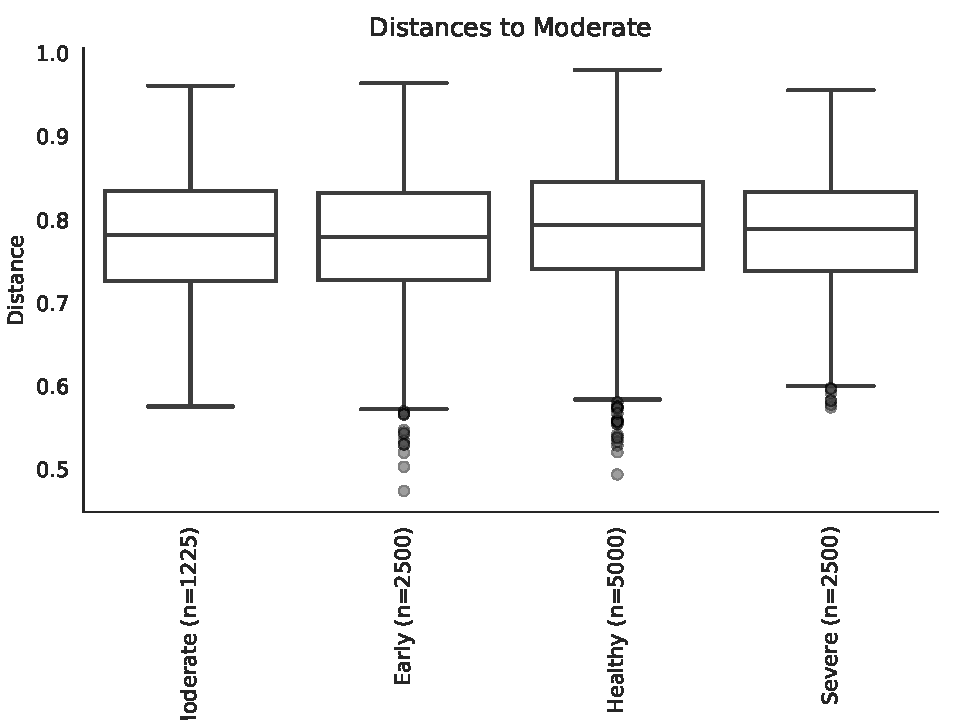
\includegraphics[width=0.25 \linewidth]{figures/BetaDiversity/DADA2/Bray/Moderate.pdf}
                &
                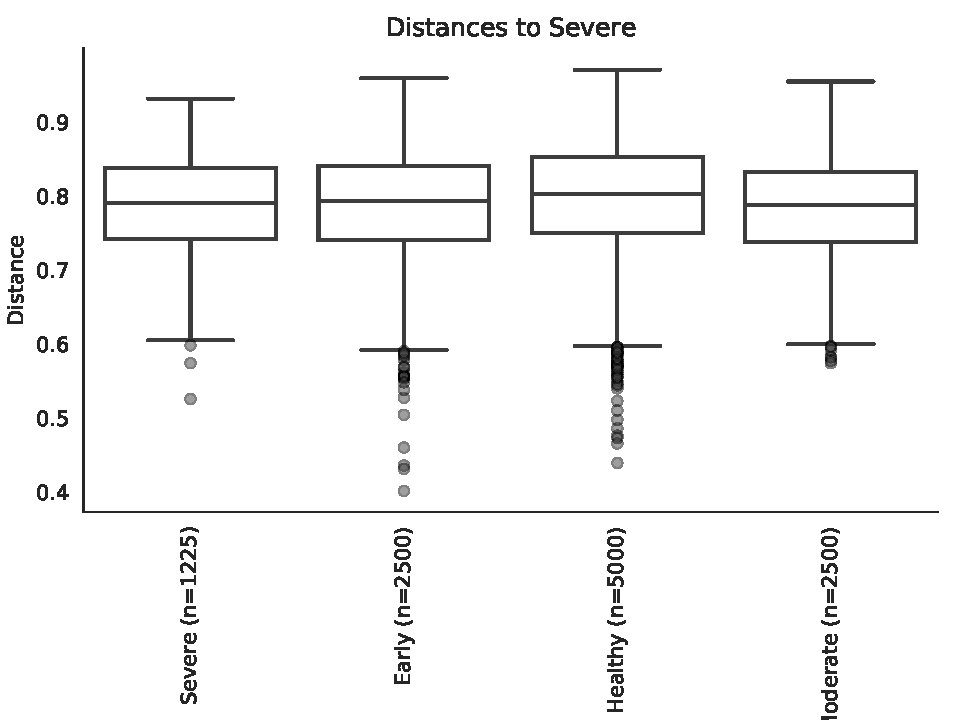
\includegraphics[width=0.25 \linewidth]{figures/BetaDiversity/DADA2/Bray/Severe.pdf}
                \\
                \mbox{(c) Moderate} & \mbox{(d) Severe} \\
            \end{array}$
            \caption{Bray-Curtis Distance with DADA2}
        \end{figure}

        \begin{figure}
            $\begin{array}{cc}
                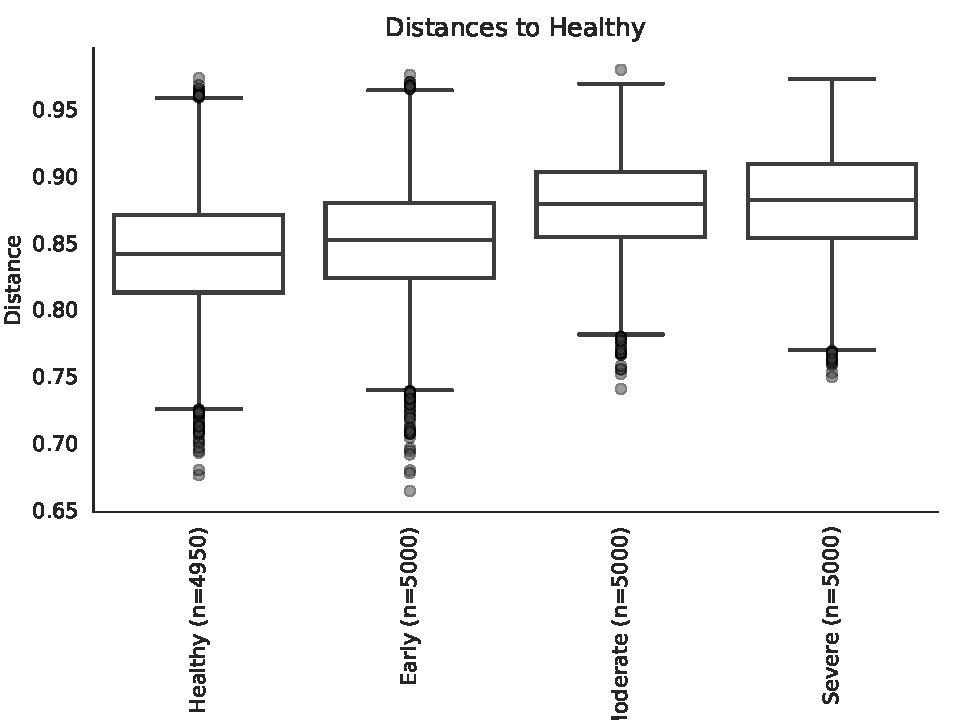
\includegraphics[width=0.25 \linewidth]{figures/BetaDiversity/DADA2/Jaccard/Healthy.pdf}
                &
                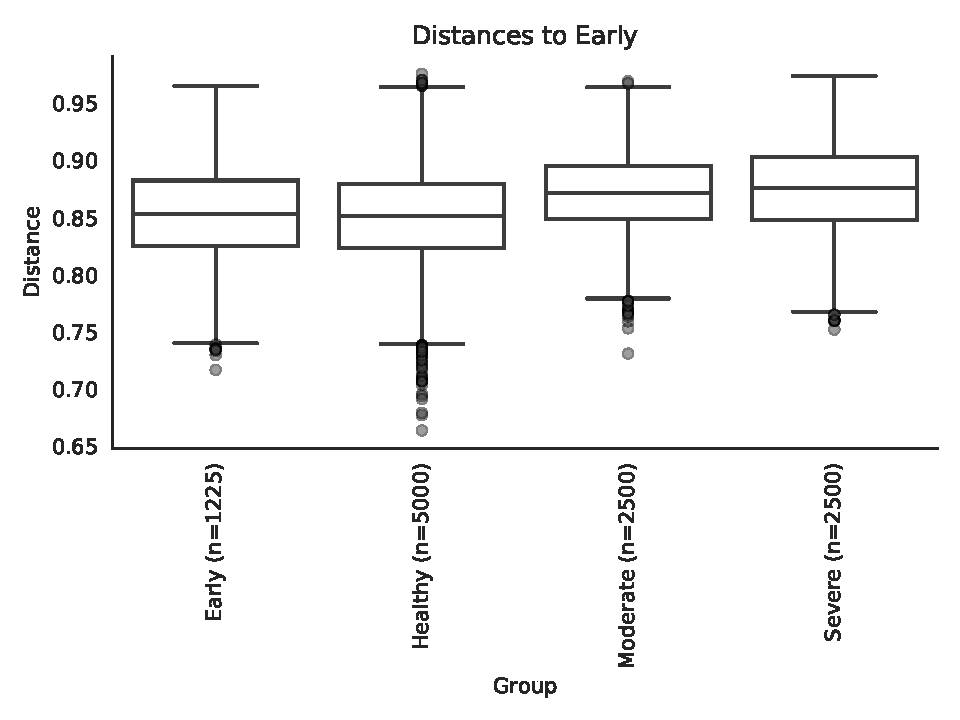
\includegraphics[width=0.25 \linewidth]{figures/BetaDiversity/DADA2/Jaccard/Early.pdf}
                \\
                \mbox{(a) Healthy} & \mbox{(b) Early} \\

                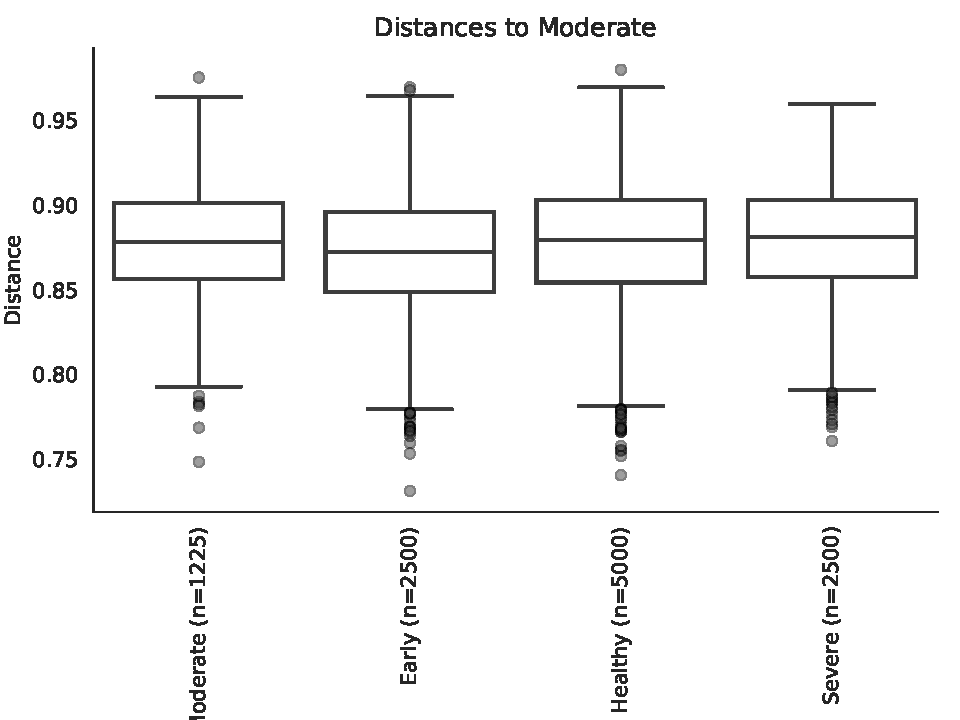
\includegraphics[width=0.25 \linewidth]{figures/BetaDiversity/DADA2/Jaccard/Moderate.pdf}
                &
                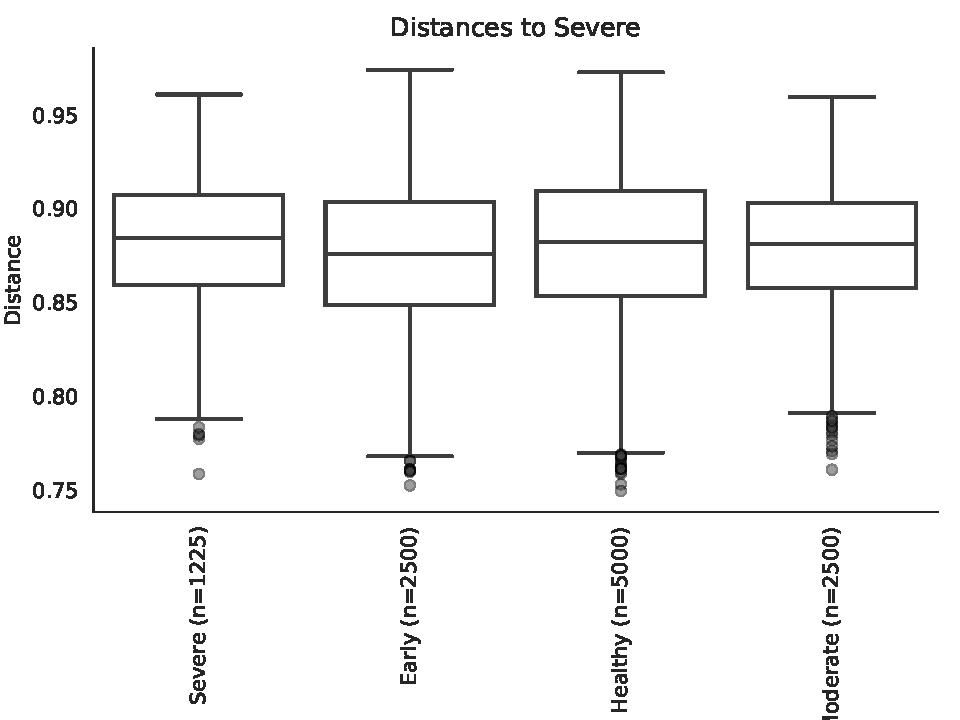
\includegraphics[width=0.25 \linewidth]{figures/BetaDiversity/DADA2/Jaccard/Severe.pdf}
                \\
                \mbox{(c) Moderate} & \mbox{(d) Severe} \\
            \end{array}$
            \caption{Jaccard Distance with DADA2}
        \end{figure}

        \begin{figure}
            $\begin{array}{cc}
                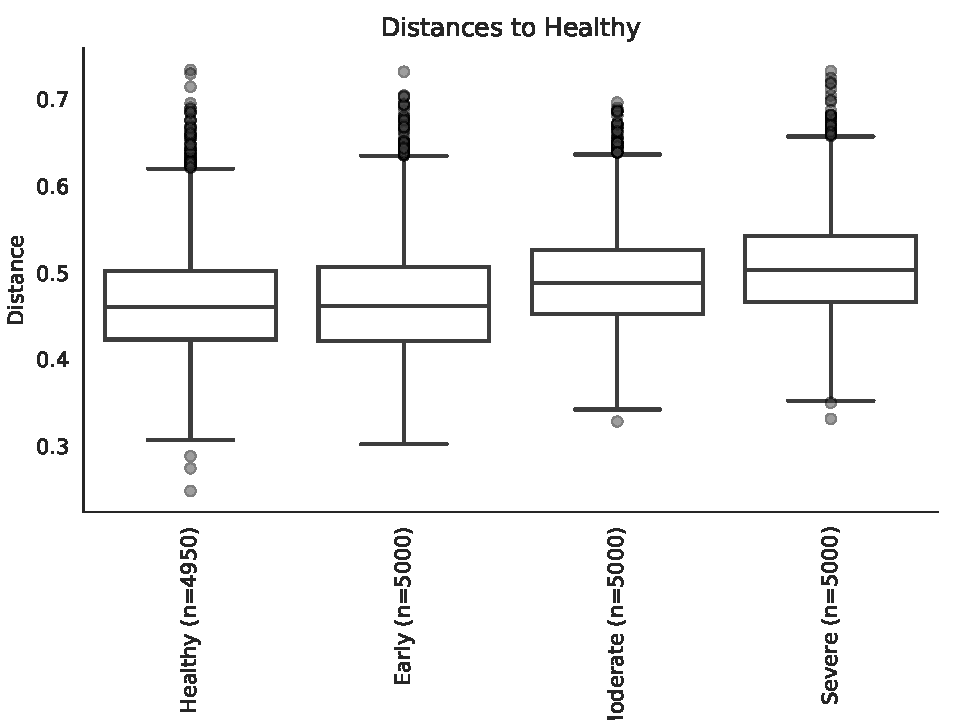
\includegraphics[width=0.25 \linewidth]{figures/BetaDiversity/DADA2/UnweightedUnifrac/Healthy.pdf}
                &
                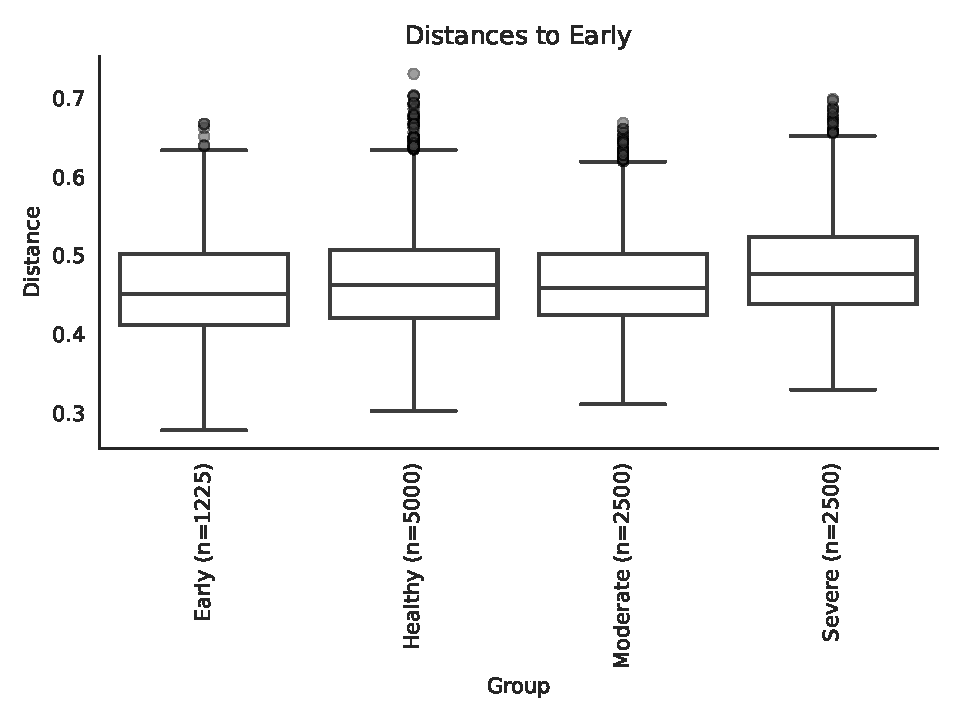
\includegraphics[width=0.25 \linewidth]{figures/BetaDiversity/DADA2/UnweightedUnifrac/Early.pdf}
                \\
                \mbox{(a) Healthy} & \mbox{(b) Early} \\

                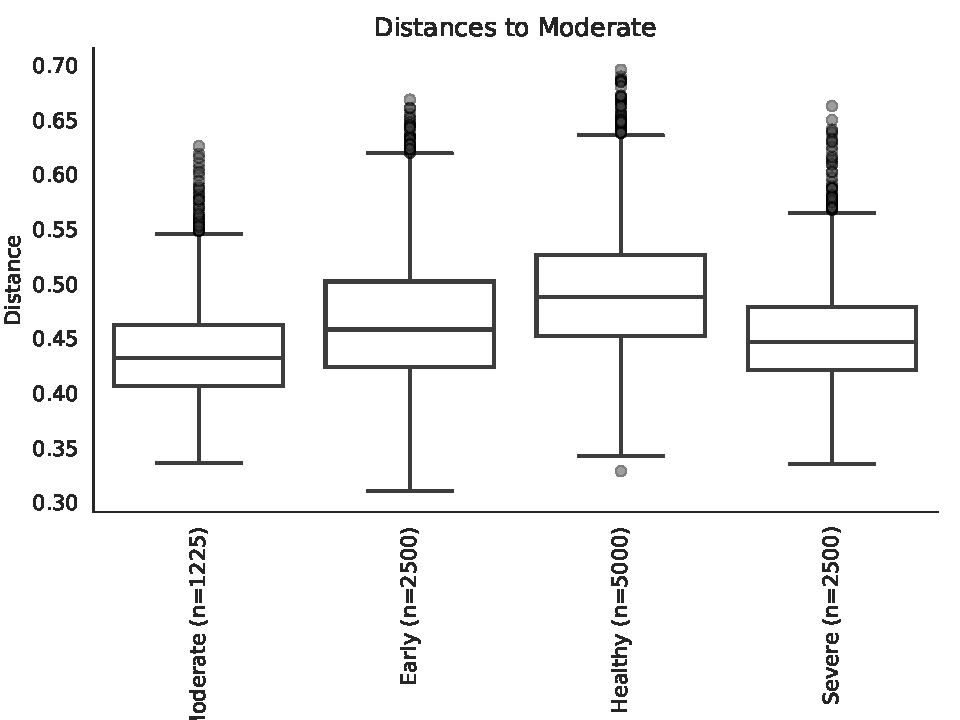
\includegraphics[width=0.25 \linewidth]{figures/BetaDiversity/DADA2/UnweightedUnifrac/Moderate.pdf}
                &
                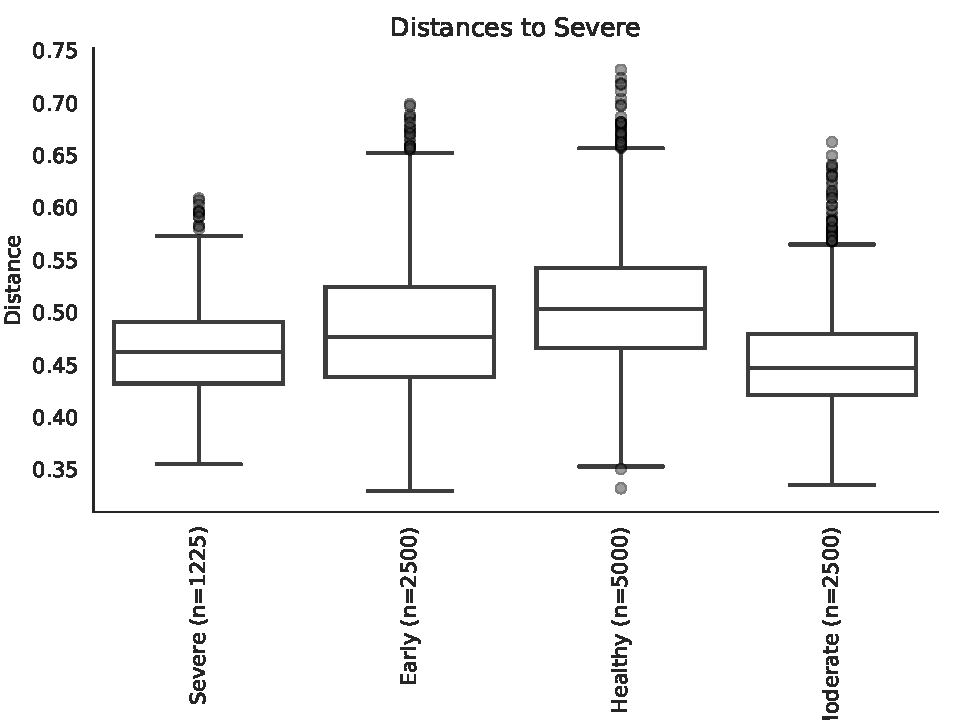
\includegraphics[width=0.25 \linewidth]{figures/BetaDiversity/DADA2/UnweightedUnifrac/Severe.pdf}
                \\
                \mbox{(c) Moderate} & \mbox{(d) Severe} \\
            \end{array}$
            \caption{Unweighted Unifrac Distance with DADA2}
        \end{figure}

        \begin{figure}
            $\begin{array}{cc}
                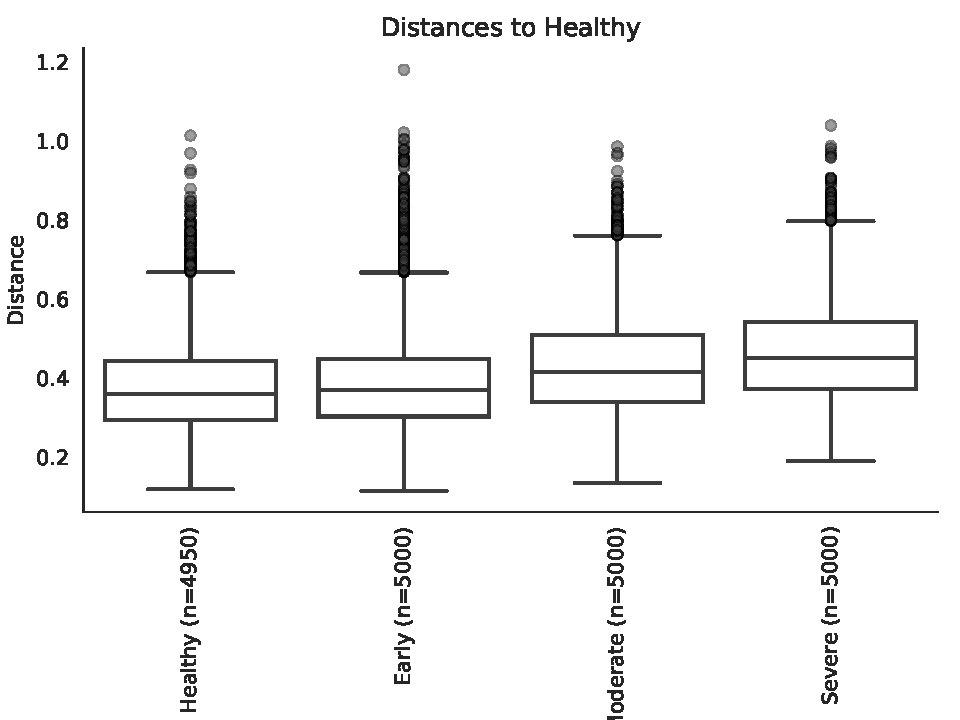
\includegraphics[width=0.25 \linewidth]{figures/BetaDiversity/DADA2/WeightedUnifrac/Healthy.pdf}
                &
                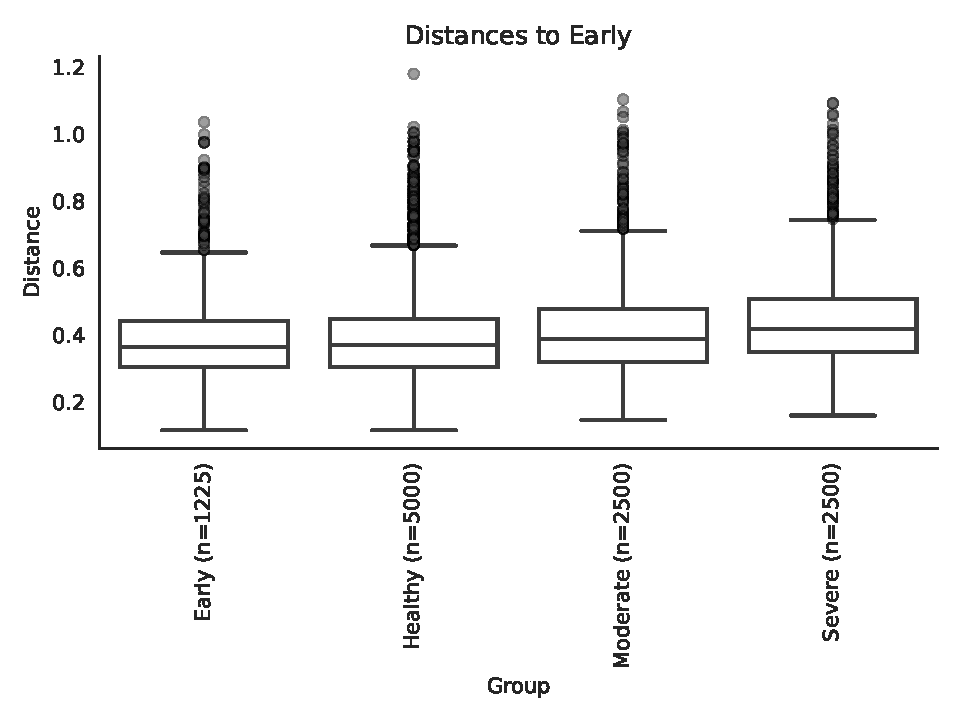
\includegraphics[width=0.25 \linewidth]{figures/BetaDiversity/DADA2/WeightedUnifrac/Early.pdf}
                \\
                \mbox{(a) Healthy} & \mbox{(b) Early} \\

                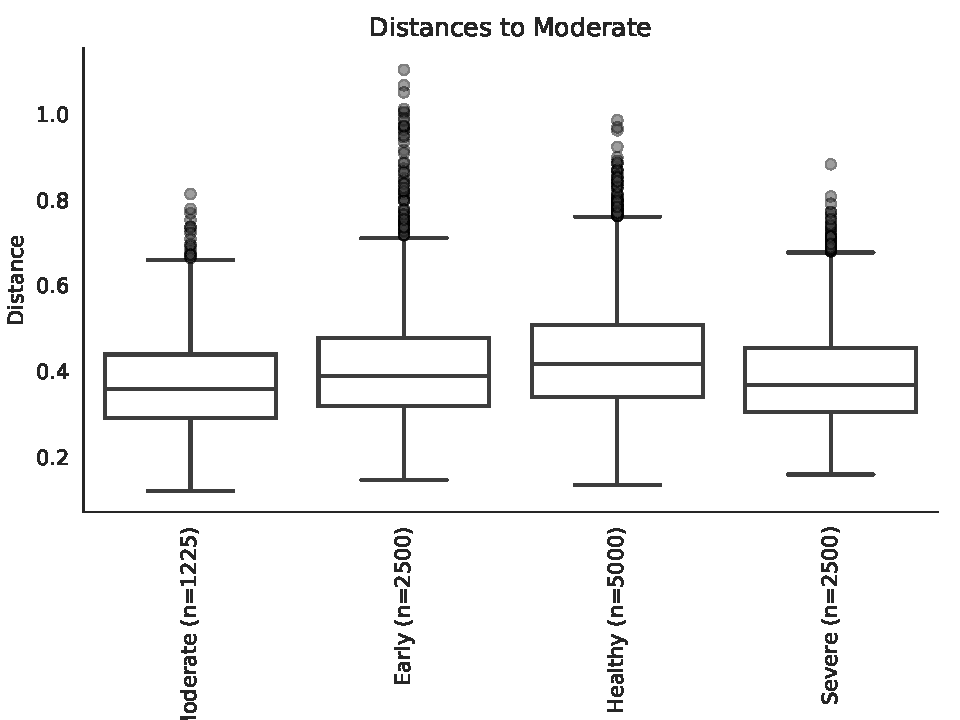
\includegraphics[width=0.25 \linewidth]{figures/BetaDiversity/DADA2/WeightedUnifrac/Moderate.pdf}
                &
                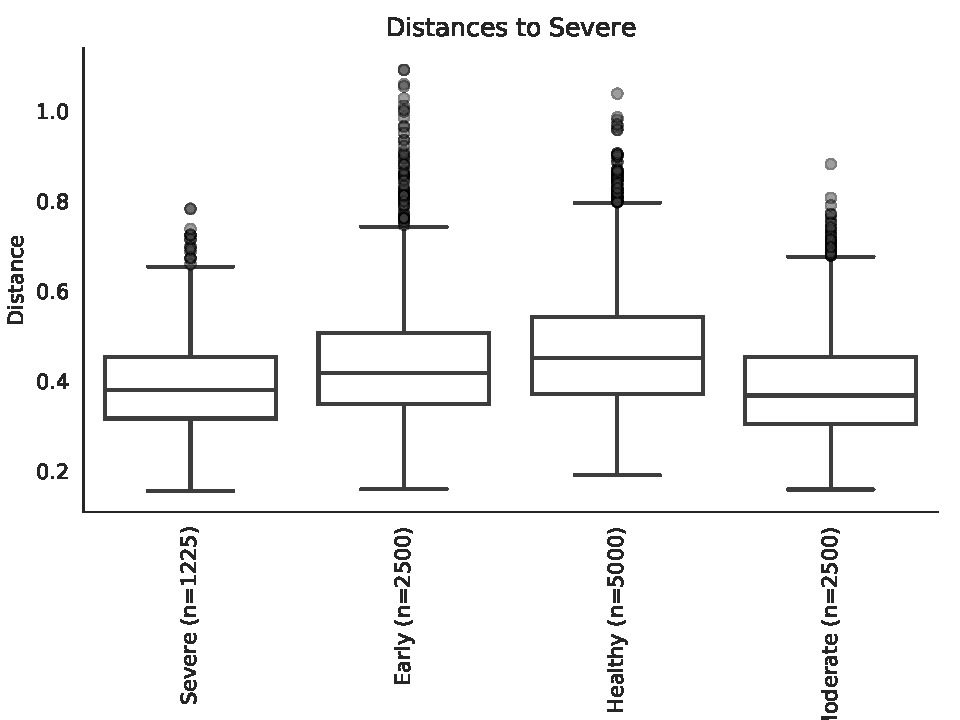
\includegraphics[width=0.25 \linewidth]{figures/BetaDiversity/DADA2/WeightedUnifrac/Severe.pdf}
                \\
                \mbox{(c) Moderate} & \mbox{(d) Severe} \\
            \end{array}$
            \caption{Weighted Unifrac Distance with DADA2}
        \end{figure}

        \begin{figure}
            $\begin{array}{cc}
                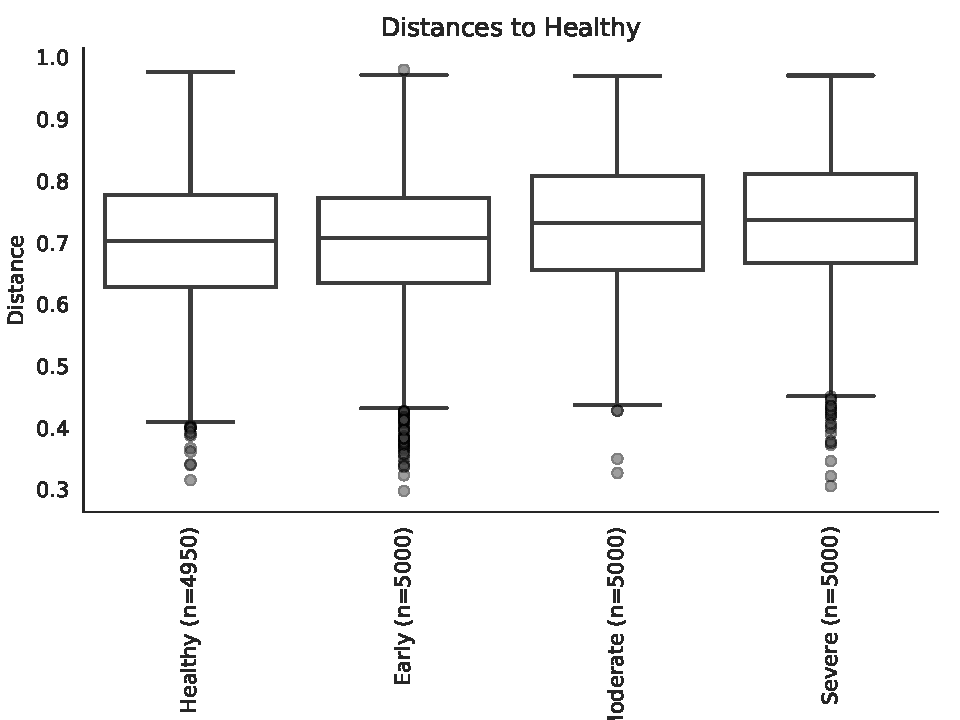
\includegraphics[width=0.25 \linewidth]{figures/BetaDiversity/Deblur/Bray/Healthy.pdf}
                &
                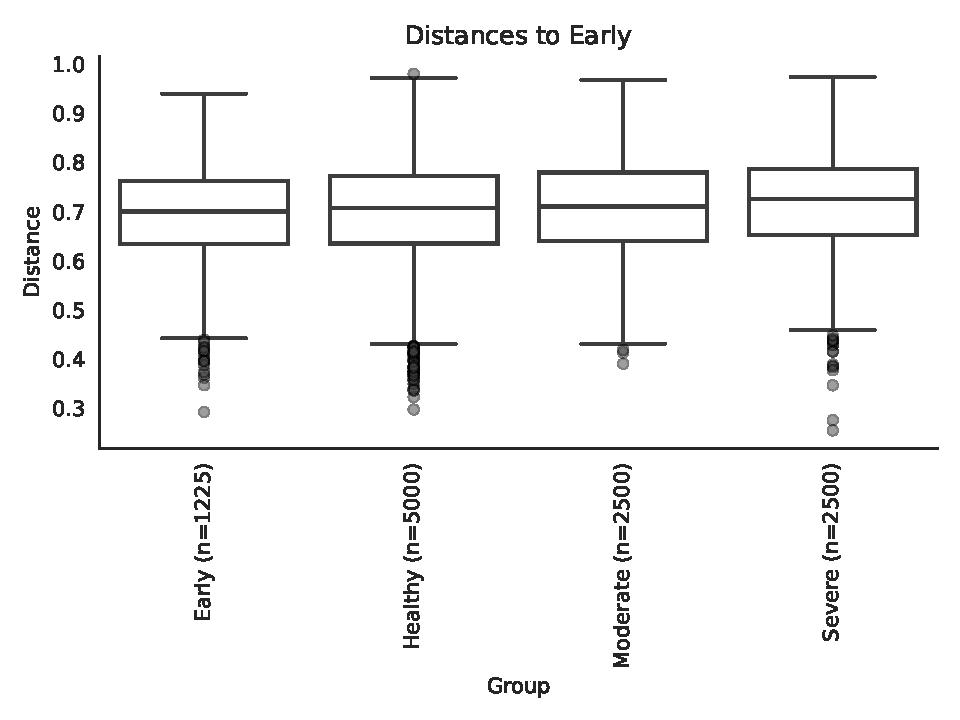
\includegraphics[width=0.25 \linewidth]{figures/BetaDiversity/Deblur/Bray/Early.pdf}
                \\
                \mbox{(a) Healthy} & \mbox{(b) Early} \\

                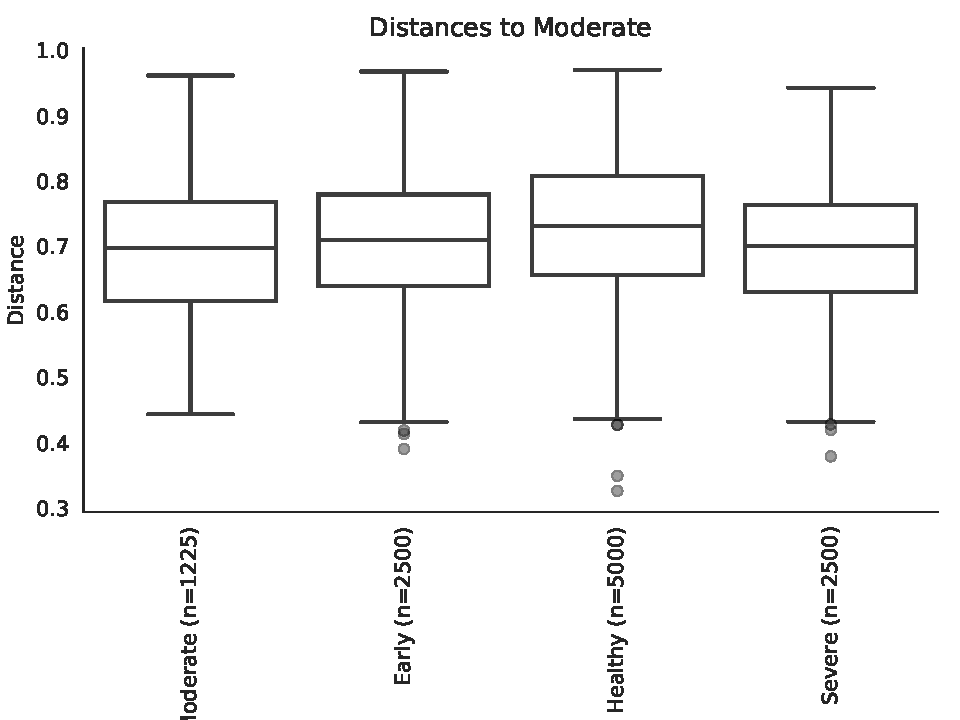
\includegraphics[width=0.25 \linewidth]{figures/BetaDiversity/Deblur/Bray/Moderate.pdf}
                &
                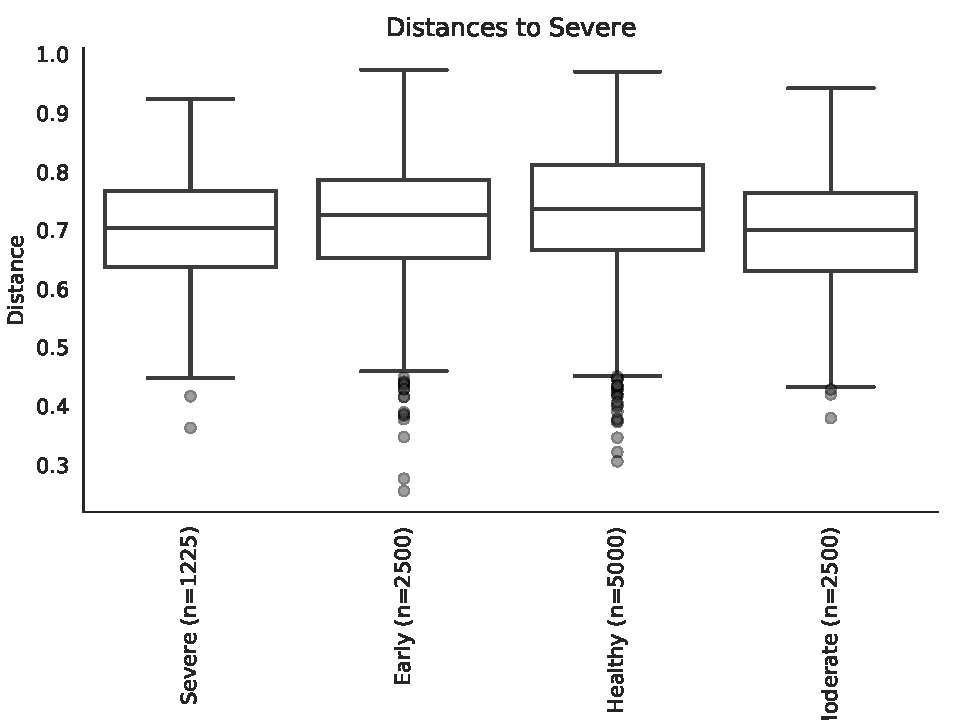
\includegraphics[width=0.25 \linewidth]{figures/BetaDiversity/Deblur/Bray/Severe.pdf}
                \\
                \mbox{(c) Moderate} & \mbox{(d) Severe} \\
            \end{array}$
            \caption{Bray-Curtis Distance with Deblur}
        \end{figure}

        \begin{figure}
            $\begin{array}{cc}
                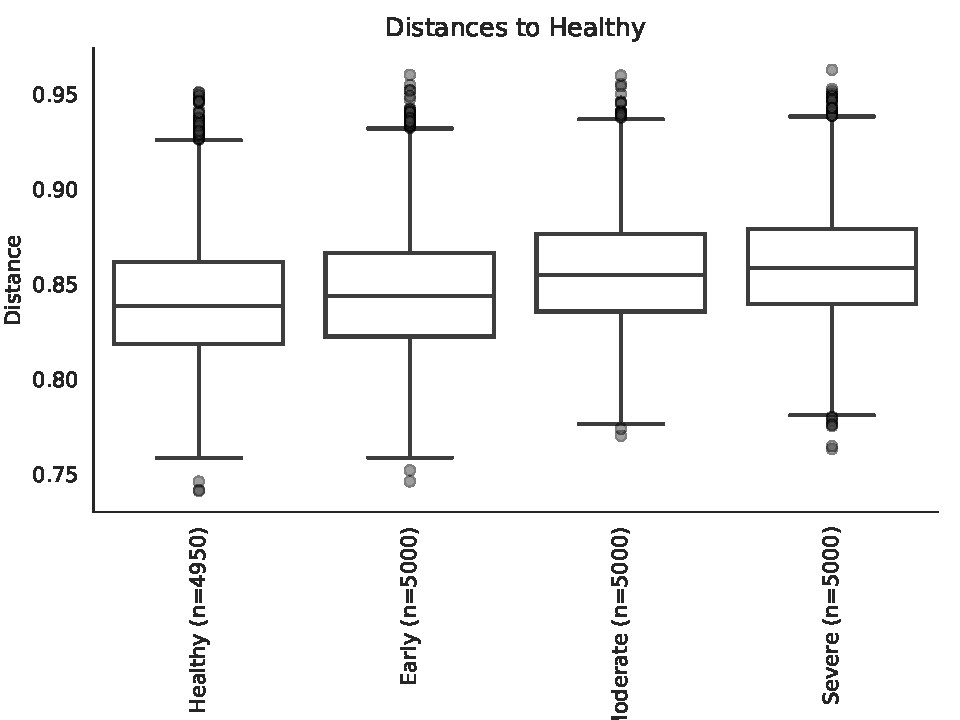
\includegraphics[width=0.25 \linewidth]{figures/BetaDiversity/Deblur/Jaccard/Healthy.pdf}
                &
                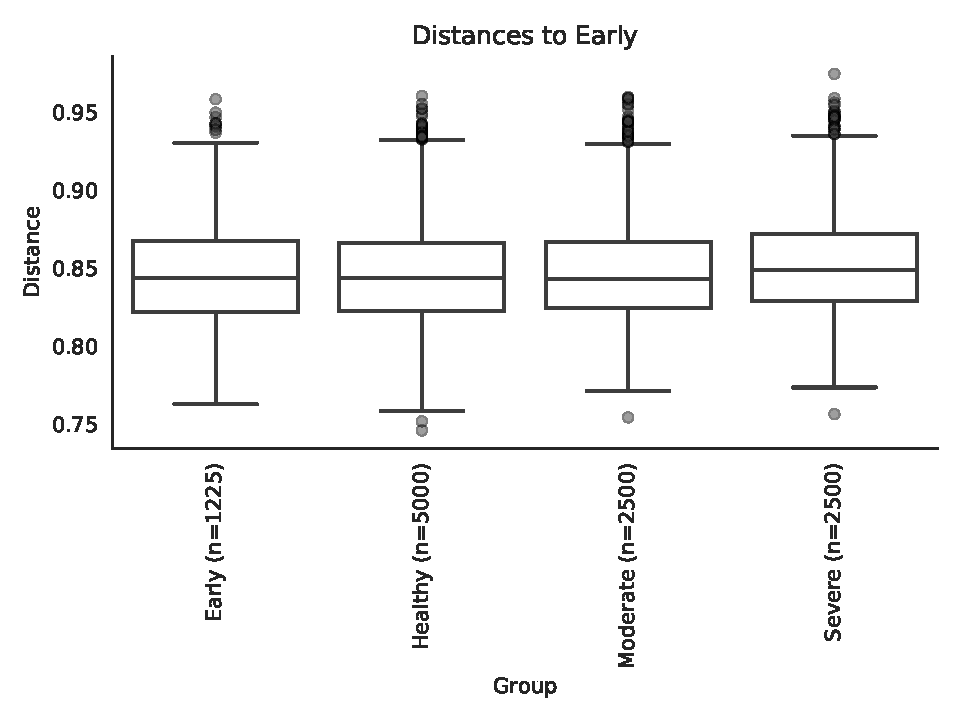
\includegraphics[width=0.25 \linewidth]{figures/BetaDiversity/Deblur/Jaccard/Early.pdf}
                \\
                \mbox{(a) Healthy} & \mbox{(b) Early} \\

                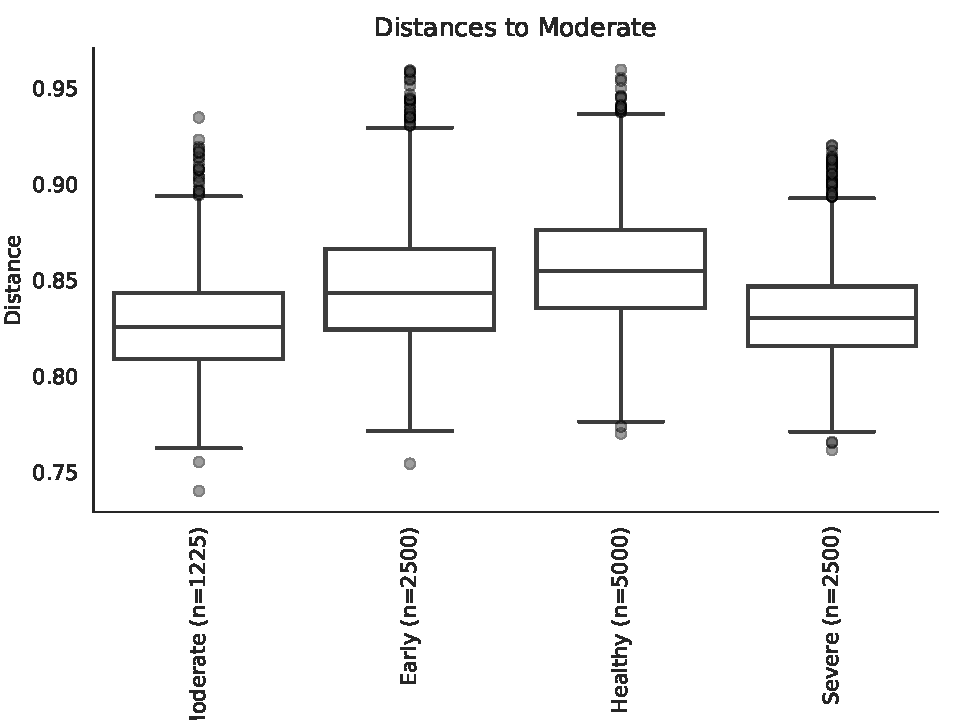
\includegraphics[width=0.25 \linewidth]{figures/BetaDiversity/Deblur/Jaccard/Moderate.pdf}
                &
                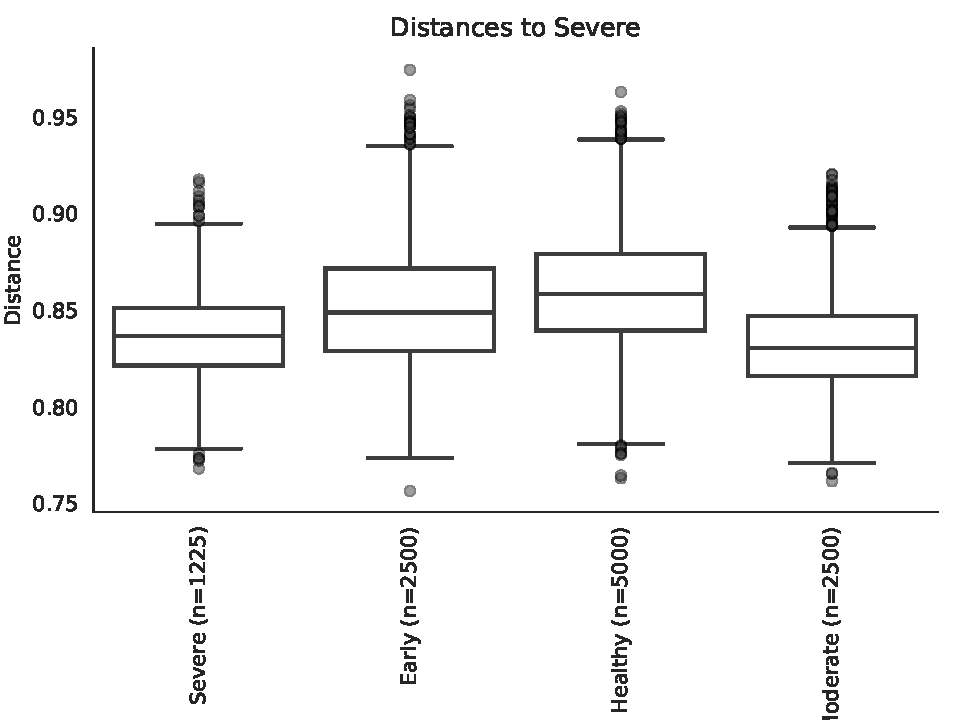
\includegraphics[width=0.25 \linewidth]{figures/BetaDiversity/Deblur/Jaccard/Severe.pdf}
                \\
                \mbox{(c) Moderate} & \mbox{(d) Severe} \\
            \end{array}$
            \caption{Jaccard Distance with Deblur}
        \end{figure}

        \begin{figure}
            $\begin{array}{cc}
                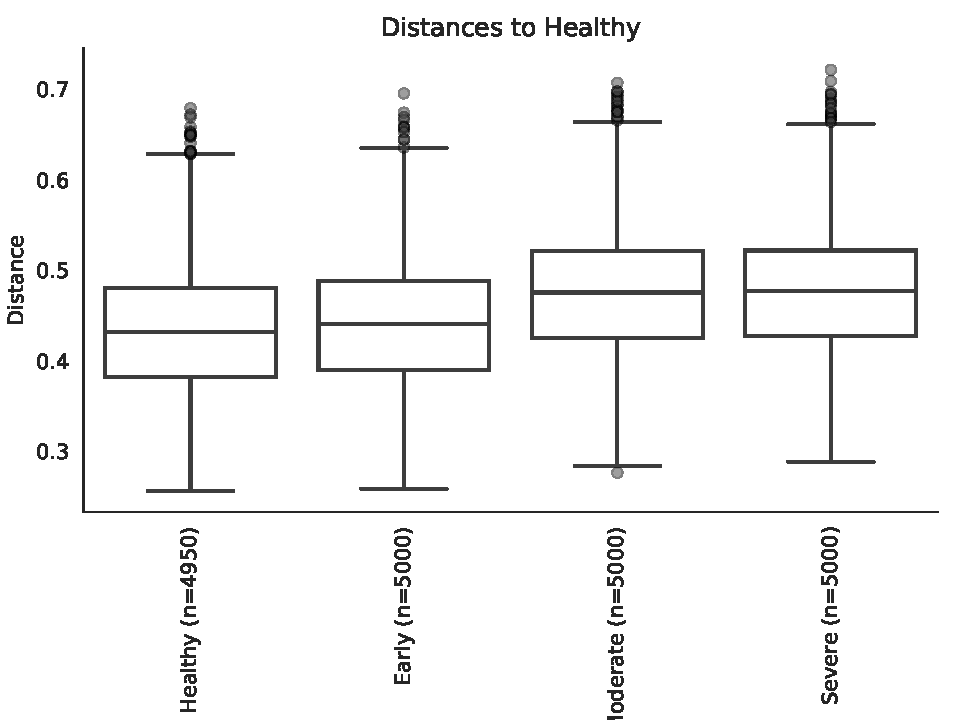
\includegraphics[width=0.25 \linewidth]{figures/BetaDiversity/Deblur/UnweightedUnifrac/Healthy.pdf}
                &
                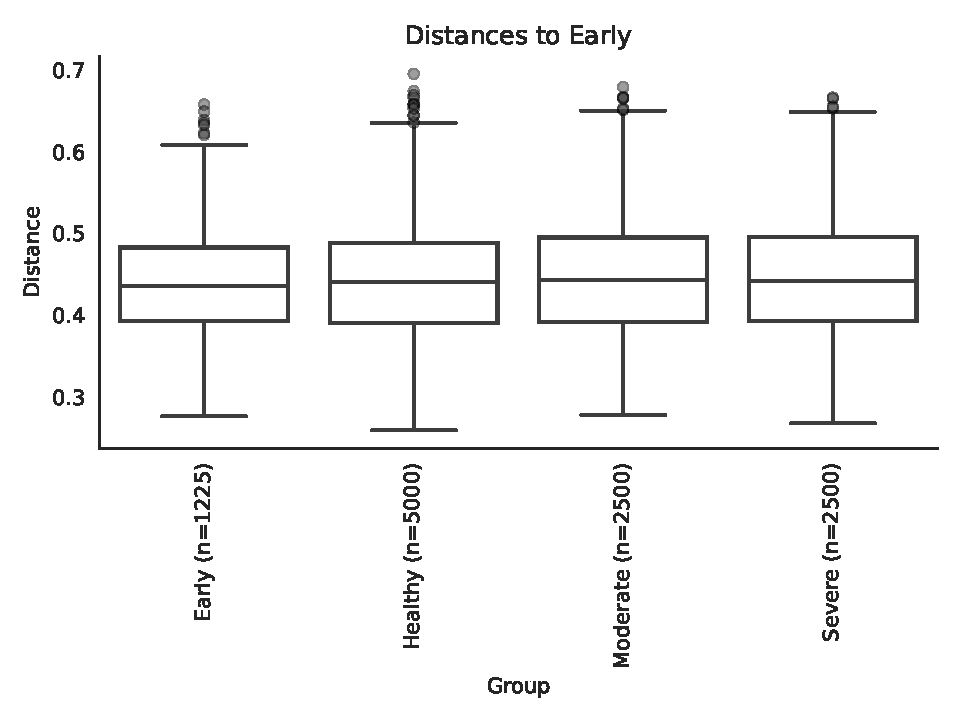
\includegraphics[width=0.25 \linewidth]{figures/BetaDiversity/Deblur/UnweightedUnifrac/Early.pdf}
                \\
                \mbox{(a) Healthy} & \mbox{(b) Early} \\

                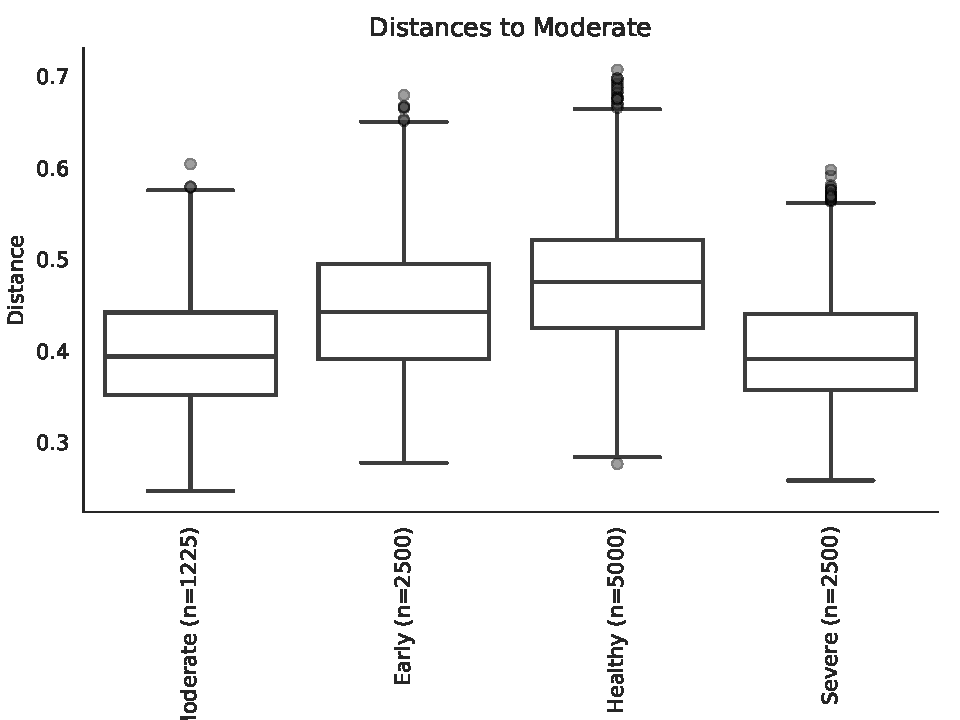
\includegraphics[width=0.25 \linewidth]{figures/BetaDiversity/Deblur/UnweightedUnifrac/Moderate.pdf}
                &
                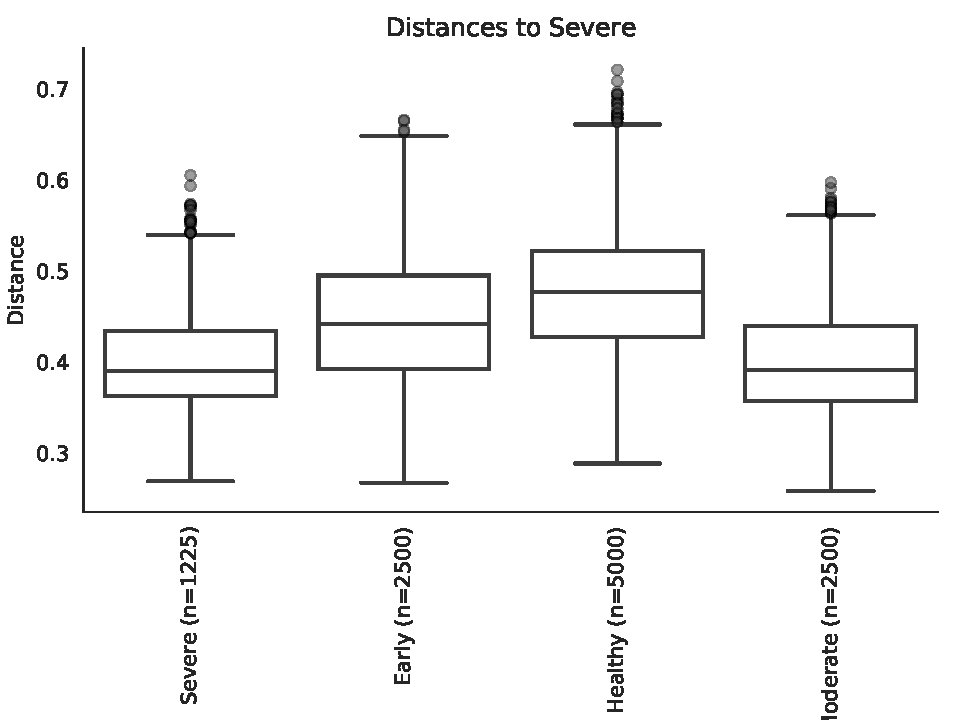
\includegraphics[width=0.25 \linewidth]{figures/BetaDiversity/Deblur/UnweightedUnifrac/Severe.pdf}
                \\
                \mbox{(c) Moderate} & \mbox{(d) Severe} \\
            \end{array}$
            \caption{Unweighted Unifrac Distance with Deblur}
        \end{figure}

        \begin{figure}
            $\begin{array}{cc}
                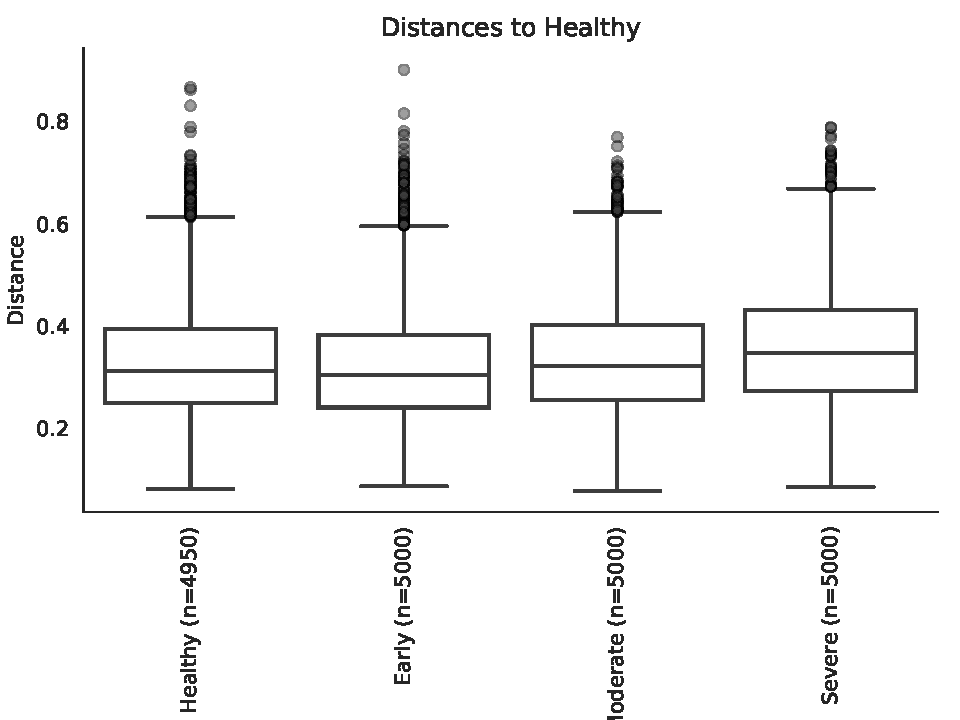
\includegraphics[width=0.25 \linewidth]{figures/BetaDiversity/Deblur/WeightedUnifrac/Healthy.pdf}
                &
                \includegraphics[width=0.25 \linewidth]{figures/BetaDiversity/Deblur/WeightedUnifrac/Early.pdf}
                \\
                \mbox{(a) Healthy} & \mbox{(b) Early} \\

                \includegraphics[width=0.25 \linewidth]{figures/BetaDiversity/Deblur/WeightedUnifrac/Moderate.pdf}
                &
                \includegraphics[width=0.25 \linewidth]{figures/BetaDiversity/Deblur/WeightedUnifrac/Severe.pdf}
                \\
                \mbox{(c) Moderate} & \mbox{(d) Severe} \\
            \end{array}$
            \caption{Weighted Unifrac Distance with Deblur}
        \end{figure}
    \end{frame}

    \begin{frame}[allowframebreaks]
        \frametitle{ANCOM}

        \begin{figure}
            $\begin{array}{cc}
                \includegraphics[width=0.4 \linewidth]{figures/ANCOM/DADA2.gg.png}
                &
                \includegraphics[width=0.4 \linewidth]{figures/ANCOM/DADA2.silva.png}
                \\
                \mbox{(a) Greengenes} & \mbox{(b) SILVA} \\
            \end{array}$
            \caption{ANCOM Volcano Plot with DADA2}
        \end{figure}

        \begin{figure}
            $\begin{array}{cc}
                \includegraphics[width=0.4 \linewidth]{figures/ANCOM/Deblur.gg.png}
                &
                \includegraphics[width=0.4 \linewidth]{figures/ANCOM/Deblur.silva.png}
                \\
                \mbox{(a) Greengenes} & \mbox{(b) SILVA} \\
            \end{array}$
            \caption{ANCOM Volcano Plot with Deblur}
        \end{figure}
    \end{frame}

    \begin{frame}[allowframebreaks]
        \frametitle{t-SNE with Whole Microbiome}

        \begin{figure}
            $\begin{array}{cc}
                \includegraphics[width=0.4 \linewidth]{figures/tSNE/Whole/whole.DADA2.gg.png}
                &
                \includegraphics[width=0.4 \linewidth]{figures/tSNE/Whole/whole.DADA2.silva.png}
                \\
                \mbox{(a) Greengenes (328 Taxa)} & \mbox{(b) SILVA (633 Taxa)}
            \end{array}$
            \caption{t-SNE Plot with Whole Microbiome from DADA2}
        \end{figure}

        \begin{figure}
            $\begin{array}{cc}
                \includegraphics[width=0.4 \linewidth]{figures/tSNE/Whole/whole.Deblur.gg.png}
                &
                \includegraphics[width=0.4 \linewidth]{figures/tSNE/Whole/whole.Deblur.silva.png}
                \\
                \mbox{(a) Greengenes (232 Taxa)} & \mbox{(b) SILVA (414 Taxa)}
            \end{array}$
            \caption{t-SNE Plot with Whole Microbiome from Deblur}
        \end{figure}
    \end{frame}

    \begin{frame}[allowframebreaks]
        \frametitle{t-SNE with ANCOM Selected}

        \begin{figure}
            $\begin{array}{cc}
                \includegraphics[width=0.4 \linewidth]{figures/tSNE/ANCOM/ANCOM.DADA2.gg.png}
                &
                \includegraphics[width=0.4 \linewidth]{figures/tSNE/ANCOM/ANCOM.DADA2.silva.png}
                \\
                \mbox{(a) Greengenes (15 Taxa)} & \mbox{(b) SILVA (23 Taxa)}
            \end{array}$
            \caption{t-SNE Plot with ANCOM Selected from DADA2}
        \end{figure}

        \begin{figure}
            $\begin{array}{cc}
                \includegraphics[width=0.4 \linewidth]{figures/tSNE/ANCOM/ANCOM.Deblur.gg.png}
                &
                \includegraphics[width=0.4 \linewidth]{figures/tSNE/ANCOM/ANCOM.Deblur.silva.png}
                \\
                \mbox{(a) Greengenes (27 Taxa)} & \mbox{(b) SILVA (20 Taxa)}
            \end{array}$
            \caption{t-SNE Plot with ANCOM Selected from Deblur}
        \end{figure}
    \end{frame}

    \begin{frame}[allowframebreaks]
        \frametitle{Random Forest Classifier}

        \begin{figure}
            \includegraphics[width=0.8 \linewidth]{figures/RandomForest/whole.pdf}
            \caption{Random Forest Classifier Workflow}
        \end{figure}

        \textbf{DADA2 + SILVA} gives the best result with many metrics.

        \begin{table}
            \caption{Features Order by Importances}
            \begin{tabular}{c|l}
                Order & Taxonomy (Genus [Species]) \\ \hline
                0 & \textit{Actinomyces} \\
                1 & \textit{Actinomyces Schaalia-odontolytica} \\
                2 & \textit{Prevotella Prevotella-intermedia} \\
                3 & \textit{Filifactor Filifactor-alocis} \\
                4 & \textit{Oribacterium} \\
                5 & \textit{Tannerella Tannerella-forsythia} \\
            \end{tabular}
        \end{table}

        \begin{figure}
            \includegraphics[width=0.8 \linewidth]{figures/RandomForest/ANCOM.DADA2.silva/balanced_accuracy.png}
            \caption{Balanced Accuracy by Feature Count}
        \end{figure}

        \begin{figure}
            \includegraphics[width=0.5 \linewidth]{figures/RandomForest/ANCOM.DADA2.silva/highest_balanced_accuracy.png}
            \caption{Random Forest Tree Plot}
        \end{figure}

        \begin{figure}
            $\begin{array}{cc}
                \includegraphics[width=0.4 \linewidth]{figures/RandomForest/ANCOM.DADA2.silva/feature_1.png}
                &
                \includegraphics[width=0.4 \linewidth]{figures/RandomForest/ANCOM.DADA2.silva/feature_2.png}
                \\
                \mbox{(a) \textit{Actinomyces}} & \mbox{(b) \textit{Actinomyces Schaalia-odontolytica}} \\
            \end{array}$
            \caption{Violin Plot by Features}
        \end{figure}
    \end{frame}

    \begin{frame}[allowframebreaks]
        \frametitle{Random Forest Classifier -- Merge Healthy+Early}

        \begin{figure}
            \includegraphics[width=0.8 \linewidth]{figures/RandomForest/merge.pdf}
            \caption{Random Forest Classifier with Merging Workflow}
        \end{figure}

        \textbf{DADA2 + GG} gives the best result with many metrics.

        \begin{table}
            \caption{Features Order by Importances}
            \begin{tabular}{c|l}
                Order & Taxonomy (Genus [Species]) \\ \hline
                0 & \textit{Actinomyces} \\
                1 & \textit{Filifactor} \\
                2 & \textit{Prevotella intermedia} \\
            \end{tabular}
        \end{table}

        \begin{figure}
            \includegraphics[width=0.8 \linewidth]{figures/RandomForest/one.DADA2.gg/balanced_accuracy.png}
            \caption{Balanced Accuracy by Feature Count}
        \end{figure}

        \begin{figure}
            \includegraphics[width=0.5 \linewidth]{figures/RandomForest/one.DADA2.gg/highest_balanced_accuracy.png}
            \caption{Random Forest Tree Plot}
        \end{figure}

        \begin{figure}
            $\begin{array}{cc}
                \includegraphics[width=0.4 \linewidth]{figures/RandomForest/one.DADA2.gg/feature_1.png}
                &
                \includegraphics[width=0.4 \linewidth]{figures/RandomForest/one.DADA2.gg/feature_2.png}
                \\
                \mbox{(a) \textit{Actinomyces}} & \mbox{(b) \textit{Filifactor}} \\
            \end{array}$
            \caption{Violin Plot by Features}
        \end{figure}
   \end{frame}

    \section{Discussion}

    \begin{frame}[allowframebreaks]
        \frametitle{References}
        \bibliographystyle{apacite}
        \bibliography{reference}
    \end{frame}
\end{document}